\chapter{HASIL DAN PEMBAHASAN}
\label{chap:hasildanpembahasan}

% Ubah bagian-bagian berikut dengan isi dari pengujian dan analisis

Pada penelitian ini dipaparkan hasil penelitian beserta analisis dari model re-identifikasi yang telah dibuat sesuai dengan 
yang telah dijelaskan pada Bab 3. Model re-identifikasi yang telah dibuat akan diujicobakan menggunakan data 
kueri dan data galeri dari dataset VRIC yang telah disiapkan. 

\section{Hasil Penelitian}
\label{sec:hasilpenelitian}

Pada penelitian ini, telah ditentukan empat jenis model re-identifikasi yang berbeda \linebreak berdasarkan jenis model dan pengaturan 
hyper-parameternya. Dan pada setiap jenis model, dilakukan tiga kali iterasi \emph{training} untuk menentukan model re-identifikasi 
terbaik di setiap jenisnya. Sehingga total model yang diciptakan pada penelitian ini berjumlah 12 model. 

Dalam proses \emph{deep learning} khususnya pada tahap \emph{training} dan \emph{validation}, terdapat nilai  akurasi, loss, dan 
nilai top 1 error, yang dapat menunjukan performa dari sebuah model saat tahapan \emph{training} dan \emph{validation} berlangsung. 
Dengan total epoch sebesar 60 untuk setiap model, akan didapatkan model dengan nilai akurasi tertinggi, dan nilai loss serta nilai 
top 1 error terendah. 

\subsection{Swin Transformer V1 Parameter 1}

Pada Swin Transformer V1 parameter 1, hyper-parameter yang ditentukan yaitu sebagai berikut:

\begin{itemize}[nolistsep]
  \item Epoch = 60
  \item Batch Size = 32
  \item Random Erasing Probability = 0
  \item Learning Rate = 0.05
  \item Warm Epoch = 0
\end{itemize}

Dengan menggunakan hyper-parameter yang ditentukan seperti diatas, dilakukan tiga kali iterasi 
\emph{training} dan \emph{validation} dengan tujuan untuk mendapatkan iterasi yang bisa memberikan 
nilai mAP dan rank@1 terbaik untuk model Swin Transformer V1 Parameter 1. Hasil Akurasi dan loss pada 
tahap \emph{training} dan \emph{validation} dapat dilihat pada tabel 
\ref{tb:NilaiakurasidanlossModelSwinTransformerV1Parameter1}.

\begin{table}[h!]
  \begin{center}
  \caption{Nilai Akurasi dan Loss Setiap Iterasi Swin Transformer V1 Parameter 1}
  \label{tb:NilaiakurasidanlossModelSwinTransformerV1Parameter1}
  \begin{tabular}{|c|c|c|c|c|}
      \hline
      \textit{ } & \begin{tabular}[c]{@{}l@{}}\textbf{Train Accuracy}\end{tabular} & \begin{tabular}[c]{@{}l@{}}\textbf{Train Loss}\end{tabular} & \begin{tabular}[c]{@{}l@{}}\textbf{Validation Accuracy}\end{tabular} & \begin{tabular}[c]{@{}l@{}}\textbf{Validation Loss}\end{tabular}\\ \hline
      \textit{\textbf{Iterasi 1}} & \begin{tabular}[c]{@{}l@{}}0.9982\end{tabular} & \begin{tabular}[c]{@{}l@{}}0.0663\end{tabular} & \begin{tabular}[c]{@{}l@{}}0.9435\end{tabular} & \begin{tabular}[c]{@{}l@{}}0.2684\end{tabular}\\ \hline
      \textit{\textbf{Iterasi 2}} & \begin{tabular}[c]{@{}l@{}}0.9979\end{tabular} & \begin{tabular}[c]{@{}l@{}}0.0658\end{tabular} & \begin{tabular}[c]{@{}l@{}}0.9453\end{tabular} & \begin{tabular}[c]{@{}l@{}}0.2725\end{tabular}\\ \hline
      \textit{\textbf{Iterasi 3}} & \begin{tabular}[c]{@{}l@{}}0.9980\end{tabular} & \begin{tabular}[c]{@{}l@{}}0.0659\end{tabular} & \begin{tabular}[c]{@{}l@{}}0.9453\end{tabular} & \begin{tabular}[c]{@{}l@{}}0.2701\end{tabular}\\ \hline
  \end{tabular}
  \end{center}
\end{table}

Selain nilai akurasi dan loss, diperoleh pula grafik loss, top 1 Error, nilai mAP, rank@1, 
rank@5, rank@10 dari proses \emph{validation} dan \emph{Testing} pada masing-masing iterasi. 
Grafik dan nilai tersebut dapat dilihat pada gambar 
\ref{fig:grafiklossdariswinv1parameter1}, gambar 
\ref{fig:grafiktop1errdariswinv1parameter1}, 
dan tabel \ref{tb:NilaimAP,Rank1,Rank5,danRank10ModelSwinTransformerV1Parameter1}.

\begin{figure}[ht]
  \centering
  % Nama dari file gambar yang diinputkan
  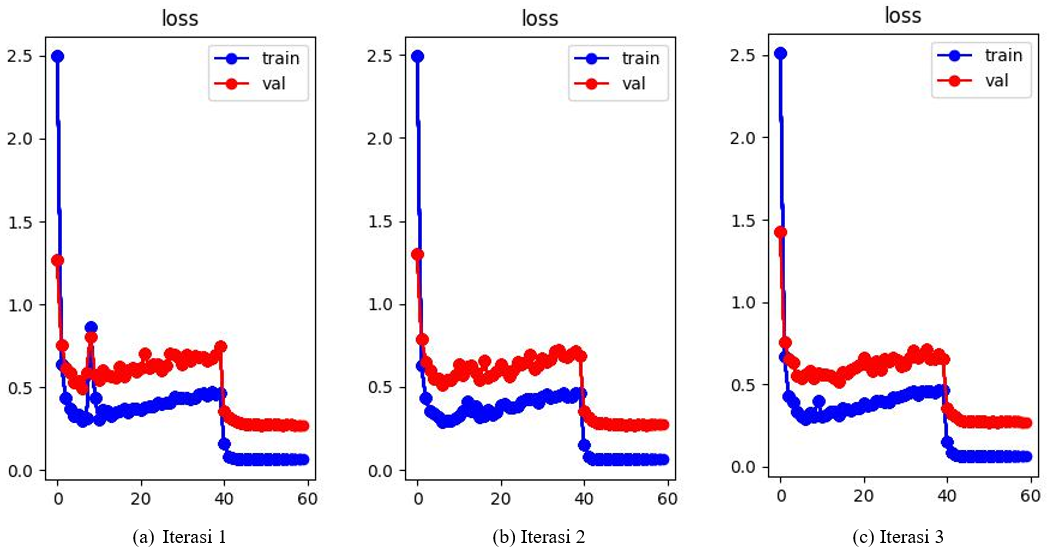
\includegraphics[scale=0.55]{gambar/Train SwinV1 Loss.png}
  % Keterangan gambar yang diinputkan
  \caption{Grafik Loss Setiap Iterasi Swin Transformer V1 Parameter 1}
  % Label referensi dari gambar yang diinputkan
  \label{fig:grafiklossdariswinv1parameter1}
\end{figure}

\begin{figure}[ht]
  \centering
  % Nama dari file gambar yang diinputkan
  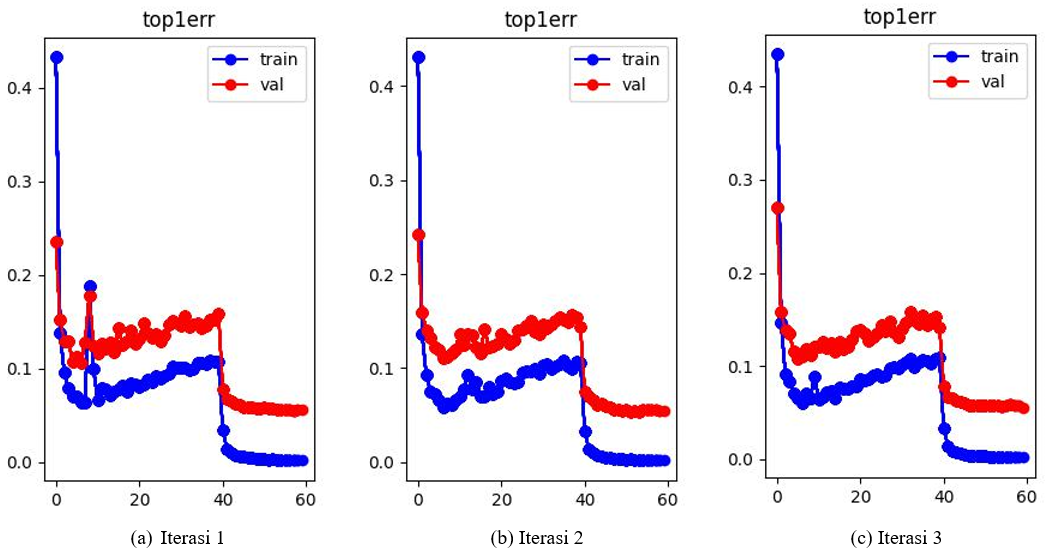
\includegraphics[scale=0.55]{gambar/Train SwinV1 Top1Err.png}
  % Keterangan gambar yang diinputkan
  \caption{Grafik Top 1 Error Setiap Iterasi Swin Transformer V1 Parameter 1}
  % Label referensi dari gambar yang diinputkan
  \label{fig:grafiktop1errdariswinv1parameter1}
\end{figure}

% Selain gambar grafik diatas, diperoleh pula nilai mAP, rank@1, rank@5, rank@10 dari proses 
% \emph{Testing} pada masing-masing iterasi. Dari tiga kali iterasi tersebut, maka didapatkan 
% rata-rata dari model Swin Transformer V1 Parameter 1. Seluruh nilai iterasi dan rata-ratanya 
% dapat dilihat pada tabel 4.1.
% Diperoleh pula nilai mAP, rank@1, rank@5, rank@10 dari proses \emph{Testing} pada 
% masing-masing iterasi. Seluruh nilai tersebut dapat dilihat di tabel 4.2.

\begin{table}[h!]
  \begin{center}
  \caption{Nilai mAP, Rank@1, Rank@5, dan Rank@10 Swin Transformer V1 Parameter 1}
  \label{tb:NilaimAP,Rank1,Rank5,danRank10ModelSwinTransformerV1Parameter1}
  \begin{tabular}{|c|c|c|c|c|}
      \hline
      \textit{ } & \begin{tabular}[c]{@{}l@{}}\textbf{mAP}\end{tabular} & \begin{tabular}[c]{@{}l@{}}\textbf{Rank@1}\end{tabular} & \begin{tabular}[c]{@{}l@{}}\textbf{Rank@5}\end{tabular} & \begin{tabular}[c]{@{}l@{}}\textbf{Rank@10}\end{tabular}\\ \hline
      \textit{\textbf{Iterasi 1}} & \begin{tabular}[c]{@{}l@{}}0.667091\end{tabular} & \begin{tabular}[c]{@{}l@{}}0.622199\end{tabular} & \begin{tabular}[c]{@{}l@{}}0.820704\end{tabular} & \begin{tabular}[c]{@{}l@{}}0.870153\end{tabular}\\ \hline
      \textit{\textbf{Iterasi 2}} & \begin{tabular}[c]{@{}l@{}}0.667997\end{tabular} & \begin{tabular}[c]{@{}l@{}}0.621487\end{tabular} & \begin{tabular}[c]{@{}l@{}}0.827819\end{tabular} & \begin{tabular}[c]{@{}l@{}}0.869086\end{tabular}\\ \hline
      \textit{\textbf{Iterasi 3}} & \begin{tabular}[c]{@{}l@{}}\textbf{0.670210}\end{tabular} & \begin{tabular}[c]{@{}l@{}}\textbf{0.623621}\end{tabular} & \begin{tabular}[c]{@{}l@{}}\textbf{0.829598}\end{tabular} & \begin{tabular}[c]{@{}l@{}}\textbf{0.872643}\end{tabular}\\ \hline
      \textit{\textbf{Rata-Rata}} & \begin{tabular}[c]{@{}l@{}}0.668432\end{tabular} & \begin{tabular}[c]{@{}l@{}}0.622435\end{tabular} & \begin{tabular}[c]{@{}l@{}}0.826040\end{tabular} & \begin{tabular}[c]{@{}l@{}}0.870627\end{tabular}\\ \hline
  \end{tabular}
  \end{center}
\end{table}

\subsection{Swin Transformer V2 Parameter 1}

Pada Swin Transformer V2 parameter 1, hyper-parameter yang ditentukan yaitu sebagai berikut:

\begin{itemize}[nolistsep]
  \item Epoch = 60
  \item Batch Size = 32
  \item Random Erasing Probability = 0
  \item Learning Rate = 0.05
  \item Warm Epoch = 0
\end{itemize}

% Dari \emph{training} dan \emph{validation}, didapatkan nilai Akurasi, nilai dan grafik loss, 
% serta grafik Top 1 Error yang dapat dilihat pada tabel 4.3, gambar 4.3, dan gambar 4.4.

% Dengan menggunakan hyper-parameter yang ditentukan seperti diatas, dilakukan tiga kali iterasi 
% \emph{training} dan \emph{validation} dengan tujuan untuk mendapatkan iterasi dengan nilai mAP \linebreak dan 
% rank@1 terbaik untuk model Swin Transformer V2 Parameter 1. Hasil Akurasi, loss, dan Top 1 Error 
% yang didapat dapat dilihat pada tabel 
% \ref{tb:NilaiakurasidanlossModelSwinTransformerV2Parameter1}, 
% gambar \ref{fig:grafiklossdantop1errdariprosestrainingdanvalidationswinv2iterasi1}, 
% dan gambar \ref{fig:grafiklossdantop1errdariprosestrainingdanvalidationswinv2iterasi2}.

Dengan menggunakan hyper-parameter yang telah ditentukan, didapatkan Hasil Akurasi, loss, dan Top 1 
Error pada tahap \emph{training} dan \emph{validation} yang dapat dilihat pada tabel 
\ref{tb:NilaiakurasidanlossModelSwinTransformerV2Parameter1}, gambar 
\ref{fig:grafiklossdariswinv2parameter1}, dan gambar 
\ref{fig:grafiktop1errdariswinv2parameter1}.

% Dengan menggunakan hyper-parameter yang ditentukan diatas, didapatkan nilai Akurasi, nilai 
% dan grafik loss, serta grafik Top 1 Error pada tahap \emph{training} dan \emph{validation} 
% yang dapat dilihat pada tabel 4.3, gambar 4.3, dan gambar 4.4.

\begin{table}[h!]
  \begin{center}
  \caption{Nilai Akurasi dan Loss Setiap Iterasi Swin Transformer V2 Parameter 1}
  \label{tb:NilaiakurasidanlossModelSwinTransformerV2Parameter1}
  \begin{tabular}{|c|c|c|c|c|}
      \hline
      \textit{ } & \begin{tabular}[c]{@{}l@{}}\textbf{Train Accuracy}\end{tabular} & \begin{tabular}[c]{@{}l@{}}\textbf{Train Loss}\end{tabular} & \begin{tabular}[c]{@{}l@{}}\textbf{Validation Accuracy}\end{tabular} & \begin{tabular}[c]{@{}l@{}}\textbf{Validation Loss}\end{tabular}\\ \hline
      \textit{\textbf{Iterasi 1}} & \begin{tabular}[c]{@{}l@{}}0.9993\end{tabular} & \begin{tabular}[c]{@{}l@{}}0.0460\end{tabular} & \begin{tabular}[c]{@{}l@{}}0.9530\end{tabular} & \begin{tabular}[c]{@{}l@{}}0.2485\end{tabular}\\ \hline
      \textit{\textbf{Iterasi 2}} & \begin{tabular}[c]{@{}l@{}}0.9993\end{tabular} & \begin{tabular}[c]{@{}l@{}}0.0462\end{tabular} & \begin{tabular}[c]{@{}l@{}}0.9567\end{tabular} & \begin{tabular}[c]{@{}l@{}}0.2361\end{tabular}\\ \hline
      \textit{\textbf{Iterasi 3}} & \begin{tabular}[c]{@{}l@{}}0.9995\end{tabular} & \begin{tabular}[c]{@{}l@{}}0.0458\end{tabular} & \begin{tabular}[c]{@{}l@{}}0.9563\end{tabular} & \begin{tabular}[c]{@{}l@{}}0.2400\end{tabular}\\ \hline
  \end{tabular}
  \end{center}
\end{table}

% Selain nilai akurasi dan loss, diperoleh pula grafik loss, top 1 Error, nilai mAP, rank@1, 
% rank@5, rank@10 dari proses \emph{Testing} dan \emph{validation} pada masing-masing iterasi. 
% Grafik dan nilai tersebut dapat dilihat pada gambar 4.3, gambar 4.4, dan tabel 4.4.

% Dengan melakukan tiga kali iterasi menggunakan hyper-parameter yang disebutkan diatas, maka didapatkan hasil berupa grafik nilai loss dan top 1 error dari proses \emph{training} dan \emph{validation} untuk model Swin Transformer V2 
% parameter 1 yang dapat dilihat pada gambar 4.3, dan gambar 4.4. Tiga kali iterasi dilakukan untuk mendapatkan 
% hasil terbaik dari model Swin Transformer V2 parameter 1.
% \\
% \\

\begin{figure}[h!]
  \centering
  % Nama dari file gambar yang diinputkan
  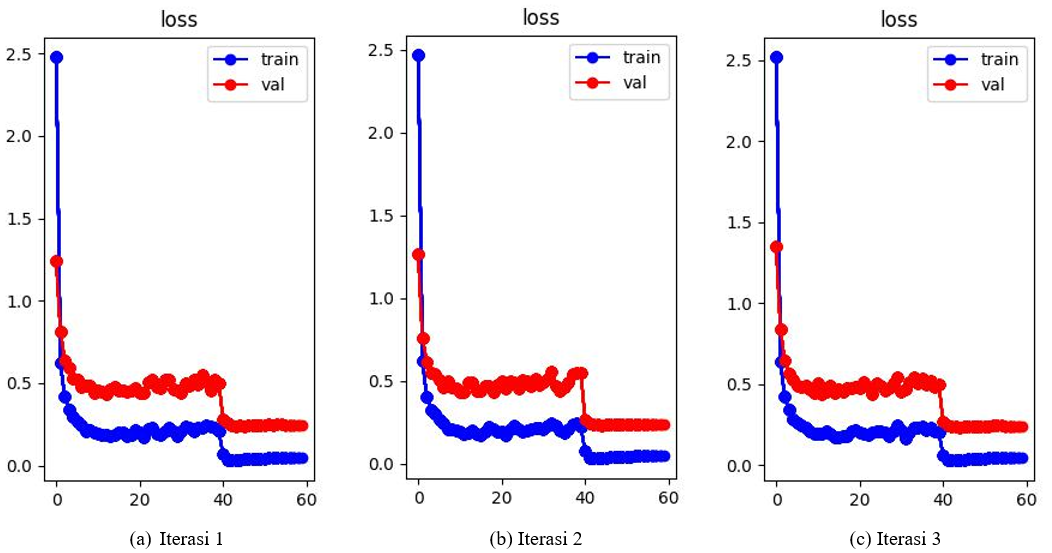
\includegraphics[scale=0.55]{gambar/Train SwinV2 Loss.png}
  % Keterangan gambar yang diinputkan
  \caption{Grafik Loss Setiap Iterasi Swin Transformer V2 Parameter 1}
  % Label referensi dari gambar yang diinputkan
  \label{fig:grafiklossdariswinv2parameter1}
\end{figure}

\begin{figure}[h!]
  \centering
  % Nama dari file gambar yang diinputkan
  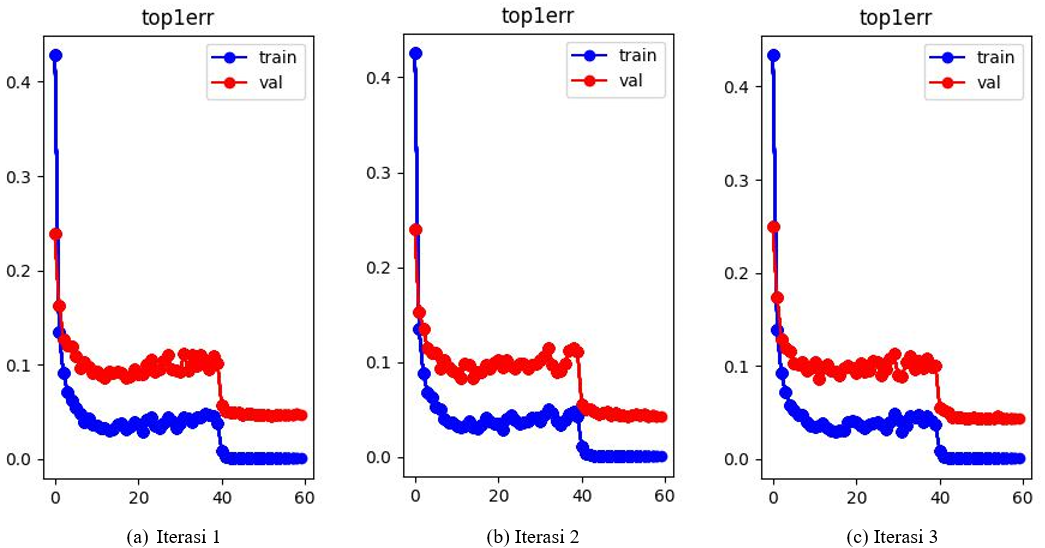
\includegraphics[scale=0.55]{gambar/Train SwinV2 Top1Err.png}
  % Keterangan gambar yang diinputkan
  \caption{Grafik Top 1 Error Setiap Iterasi Swin Transformer V2 Parameter 1}
  % Label referensi dari gambar yang diinputkan
  \label{fig:grafiktop1errdariswinv2parameter1}
\end{figure}

Selain nilai akurasi, loss, dan Top 1 Error, diperoleh pula nilai mAP, rank@1, 
rank@5, rank@10 dari proses \emph{validation} dan \emph{Testing} pada 
masing-masing iterasi. Grafik dan nilai tersebut dapat dilihat pada tabel 
\ref{tb:NilaimAP,Rank1,Rank5,danRank10ModelSwinTransformerV2Parameter1}.

% Diperoleh pula nilai mAP, rank@1, rank@5, rank@10 dari proses \emph{Testing} pada 
% masing-masing iterasi. Seluruh nilai tersebut dapat dilihat di tabel 4.5.

\begin{table}[h!]
  \begin{center}
  \caption{Nilai mAP, Rank@1, Rank@5, dan Rank@10 Swin Transformer V2 Parameter 1}
  \label{tb:NilaimAP,Rank1,Rank5,danRank10ModelSwinTransformerV2Parameter1}
  \begin{tabular}{|c|c|c|c|c|}
      \hline
      \textit{ } & \begin{tabular}[c]{@{}l@{}}\textbf{mAP}\end{tabular} & \begin{tabular}[c]{@{}l@{}}\textbf{Rank@1}\end{tabular} & \begin{tabular}[c]{@{}l@{}}\textbf{Rank@5}\end{tabular} & \begin{tabular}[c]{@{}l@{}}\textbf{Rank@10}\end{tabular}\\ \hline
      \textit{\textbf{Iterasi 1}} & \begin{tabular}[c]{@{}l@{}}\textbf{0.725377}\end{tabular} & \begin{tabular}[c]{@{}l@{}}\textbf{0.686233}\end{tabular} & \begin{tabular}[c]{@{}l@{}}0.857346\end{tabular} & \begin{tabular}[c]{@{}l@{}}0.895411\end{tabular}\\ \hline
      \textit{\textbf{Iterasi 2}} & \begin{tabular}[c]{@{}l@{}}0.719978\end{tabular} & \begin{tabular}[c]{@{}l@{}}0.678762\end{tabular} & \begin{tabular}[c]{@{}l@{}}\textbf{0.863750}\end{tabular} & \begin{tabular}[c]{@{}l@{}}\textbf{0.903949}\end{tabular}\\ \hline
      \textit{\textbf{Iterasi 3}} & \begin{tabular}[c]{@{}l@{}}0.717680\end{tabular} & \begin{tabular}[c]{@{}l@{}}0.676272\end{tabular} & \begin{tabular}[c]{@{}l@{}}0.857702\end{tabular} & \begin{tabular}[c]{@{}l@{}}0.900747\end{tabular}\\ \hline
      \textit{\textbf{Rata-Rata}} & \begin{tabular}[c]{@{}l@{}}0,721011\end{tabular} & \begin{tabular}[c]{@{}l@{}}0,680422\end{tabular} & \begin{tabular}[c]{@{}l@{}}0,859599\end{tabular} & \begin{tabular}[c]{@{}l@{}}0,900035\end{tabular}\\ \hline
  \end{tabular}
  \end{center}
\end{table}

\subsection{Swin Transformer V1 Parameter 2}

Pada Swin Transformer V1 parameter 2, hyper-parameter yang ditentukan yaitu:

\begin{itemize}[nolistsep]
  \item Epoch = 60
  \item Batch Size = 16
  \item Random Erasing Probability = 0.5
  \item Learning Rate = 0.01
  \item Warm Epoch = 5
\end{itemize}

Dengan menggunakan hyper-parameter yang telah ditentukan, didapatkan Hasil Akurasi, loss, dan Top 1 
Error yang dapat dilihat pada tabel 
\ref{tb:NilaiakurasidanlossModelSwinTransformerV1Parameter2}, gambar 
\ref{fig:grafiklossdariswinv1parameter2}, dan gambar \ref{fig:grafiktop1errdariswinv1parameter2}.

% Dengan menggunakan hyper-parameter yang ditentukan seperti diatas, dilakukan tiga kali iterasi 
% \emph{training} dan \emph{validation} dengan tujuan untuk mendapatkan iterasi dengan nilai mAP dan 
% rank@1 terbaik untuk model Swin Transformer V1 Parameter 2. Hasil Akurasi dan loss pada tahap 
% \emph{training} dan \emph{validation} dapat dilihat pada tabel 4.5.

\begin{table}[h!]
  \begin{center}
  \caption{Nilai Akurasi dan Loss Setiap Iterasi Swin Transformer V1 Parameter 2}
  \label{tb:NilaiakurasidanlossModelSwinTransformerV1Parameter2}
  \begin{tabular}{|c|c|c|c|c|}
      \hline
      \textit{ } & \begin{tabular}[c]{@{}l@{}}\textbf{Train Accuracy}\end{tabular} & \begin{tabular}[c]{@{}l@{}}\textbf{Train Loss}\end{tabular} & \begin{tabular}[c]{@{}l@{}}\textbf{Validation Accuracy}\end{tabular} & \begin{tabular}[c]{@{}l@{}}\textbf{Validation Loss}\end{tabular}\\ \hline
      \textit{\textbf{Iterasi 1}} & \begin{tabular}[c]{@{}l@{}}0.9979\end{tabular} & \begin{tabular}[c]{@{}l@{}}0.1139\end{tabular} & \begin{tabular}[c]{@{}l@{}}0.9571\end{tabular} & \begin{tabular}[c]{@{}l@{}}0.1969\end{tabular}\\ \hline
      \textit{\textbf{Iterasi 2}} & \begin{tabular}[c]{@{}l@{}}0.9980\end{tabular} & \begin{tabular}[c]{@{}l@{}}0.1196\end{tabular} & \begin{tabular}[c]{@{}l@{}}0.9578\end{tabular} & \begin{tabular}[c]{@{}l@{}}0.1897\end{tabular}\\ \hline
      \textit{\textbf{Iterasi 3}} & \begin{tabular}[c]{@{}l@{}}0.9985\end{tabular} & \begin{tabular}[c]{@{}l@{}}0.1180\end{tabular} & \begin{tabular}[c]{@{}l@{}}0.9563\end{tabular} & \begin{tabular}[c]{@{}l@{}}0.1847\end{tabular}\\ \hline
  \end{tabular}
  \end{center}
\end{table}

% Selain nilai akurasi dan loss, diperoleh pula grafik loss, grafik Top 1 Error, nilai mAP, rank@1, 
% rank@5, dan rank@10 dari proses \emph{Testing} dan \emph{validation} pada masing-masing iterasi. 
% Grafik dan nilai tersebut dapat dilihat pada gambar 4.5, gambar 4.6, dan tabel 4.6.

\begin{figure}[h!]
  \centering
  % Nama dari file gambar yang diinputkan
  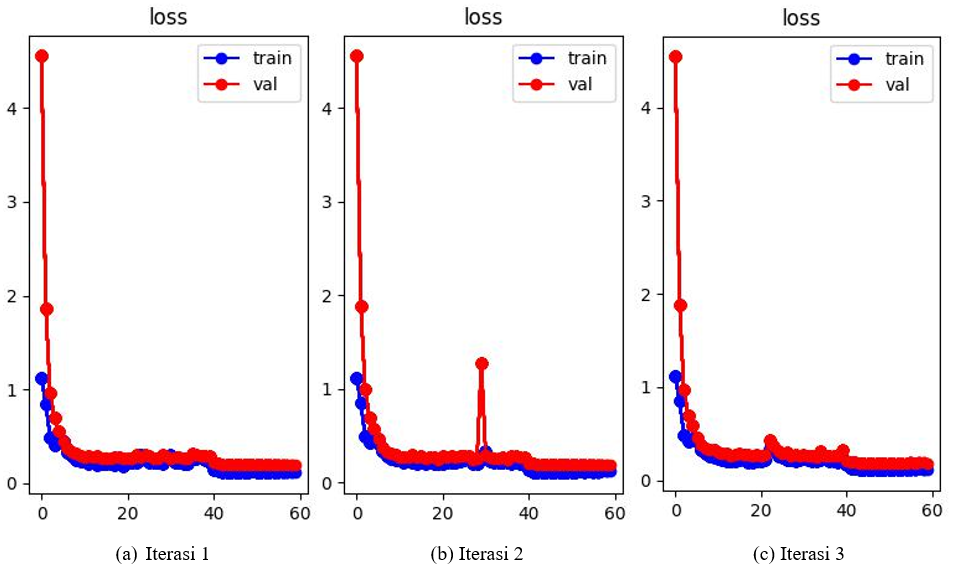
\includegraphics[scale=0.55]{gambar/Train SwinV1CP1 Loss.png}
  % Keterangan gambar yang diinputkan
  \caption{Grafik Loss Setiap Iterasi Swin Transformer V1 Parameter 2}
  % Label referensi dari gambar yang diinputkan
  \label{fig:grafiklossdariswinv1parameter2}
\end{figure}

\begin{figure}[h!]
  \centering
  % Nama dari file gambar yang diinputkan
  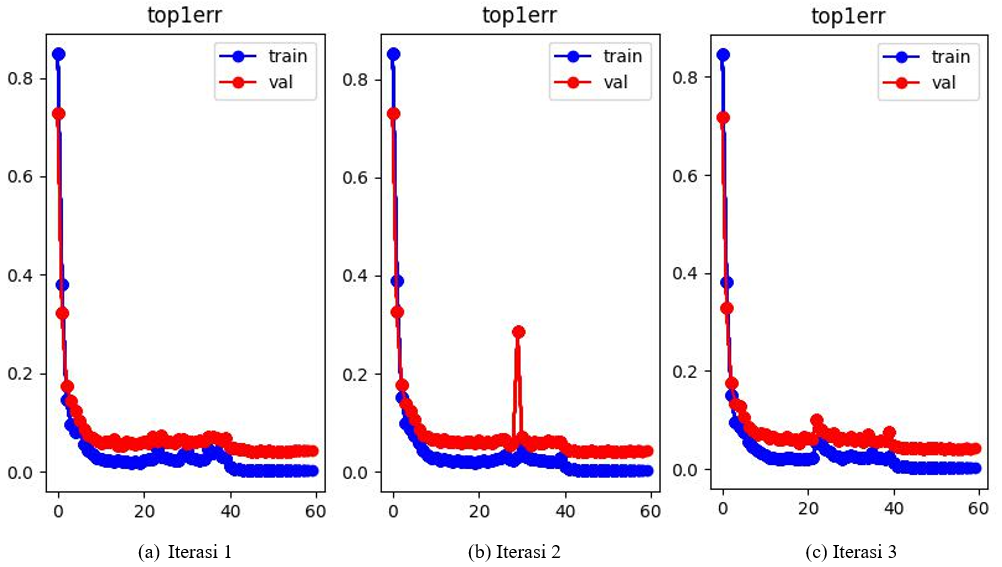
\includegraphics[scale=0.55]{gambar/Train SwinV1CP1 Top1Err.png}
  % Keterangan gambar yang diinputkan
  \caption{Grafik Top 1 Error Setiap Iterasi Swin Transformer V1 Parameter 2}
  % Label referensi dari gambar yang diinputkan
  \label{fig:grafiktop1errdariswinv1parameter2}
\end{figure}

% Selain gambar grafik diatas, diperoleh pula nilai mAP, rank@1, rank@5, rank@10 dari proses 
% \emph{Testing} pada masing-masing iterasi. Dari tiga kali iterasi tersebut, maka didapatkan 
% rata-rata dari model Swin Transformer V1 Parameter 1. Seluruh nilai iterasi dan rata-ratanya 
% dapat dilihat pada tabel 4.1.
% Diperoleh pula nilai mAP, rank@1, rank@5, rank@10 dari proses \emph{Testing} pada 
% masing-masing iterasi. Seluruh nilai tersebut dapat dilihat di tabel 4.2.

Kemudian diperoleh pula nilai mAP, rank@1, rank@5, dan rank@10 dari proses \emph{Testing} 
dan \emph{validation} pada masing-masing iterasi yang dapat dilihat pada 
tabel \ref{tb:NilaimAP,Rank1,Rank5,danRank10ModelSwinTransformerV1Parameter2}.

\begin{table}[h!]
  \begin{center}
  \caption{Nilai mAP, Rank@1, Rank@5, dan Rank@10 Swin Transformer V1 Parameter 2}
  \label{tb:NilaimAP,Rank1,Rank5,danRank10ModelSwinTransformerV1Parameter2}
  \begin{tabular}{|c|c|c|c|c|}
      \hline
      \textit{ } & \begin{tabular}[c]{@{}l@{}}\textbf{mAP}\end{tabular} & \begin{tabular}[c]{@{}l@{}}\textbf{Rank@1}\end{tabular} & \begin{tabular}[c]{@{}l@{}}\textbf{Rank@5}\end{tabular} & \begin{tabular}[c]{@{}l@{}}\textbf{Rank@10}\end{tabular}\\ \hline
      \textit{\textbf{Iterasi 1}} & \begin{tabular}[c]{@{}l@{}}0.743027\end{tabular} & \begin{tabular}[c]{@{}l@{}}0.701530\end{tabular} & \begin{tabular}[c]{@{}l@{}}0.885094\end{tabular} & \begin{tabular}[c]{@{}l@{}}0.925294\end{tabular}\\ \hline
      \textit{\textbf{Iterasi 2}} & \begin{tabular}[c]{@{}l@{}}\textbf{0.748120}\end{tabular} & \begin{tabular}[c]{@{}l@{}}\textbf{0.706866}\end{tabular} & \begin{tabular}[c]{@{}l@{}}\textbf{0.890786}\end{tabular} & \begin{tabular}[c]{@{}l@{}}0.932053\end{tabular}\\ \hline
      \textit{\textbf{Iterasi 3}} & \begin{tabular}[c]{@{}l@{}}0.748066\end{tabular} & \begin{tabular}[c]{@{}l@{}}0.706510\end{tabular} & \begin{tabular}[c]{@{}l@{}}0.890430\end{tabular} & \begin{tabular}[c]{@{}l@{}}\textbf{0.934543}\end{tabular}\\ \hline
      \textit{\textbf{Rata-Rata}} & \begin{tabular}[c]{@{}l@{}}0,746404\end{tabular} & \begin{tabular}[c]{@{}l@{}}0,705640\end{tabular} & \begin{tabular}[c]{@{}l@{}}0.888770\end{tabular} & \begin{tabular}[c]{@{}l@{}}0,930630\end{tabular}\\ \hline
  \end{tabular}
  \end{center}
\end{table}

\subsection{Swin Transformer V2 Parameter 2}

Pada Swin Transformer V2 parameter 2, hyper-parameter yang ditentukan yaitu:

\begin{itemize}[nolistsep]
  \item Epoch = 60
  \item Batch Size = 16
  \item Random Erasing Probability = 0.5
  \item Learning Rate = 0.01
  \item Warm Epoch = 5
\end{itemize}

Dengan menggunakan hyper-parameter yang ditentukan seperti diatas, didapatkan hasil akurasi, loss, 
dan Top 1 Error pada tahap \emph{training} dan \emph{validation} yang dapat dilihat pada 
tabel \ref{tb:NilaiakurasidanlossModelSwinTransformerV2Parameter2}, gambar 
\ref{fig:grafiklossdariswinv2parameter2} dan gambar \ref{fig:grafiktop1errdariswinv2parameter2}.

\begin{table}[h!]
  \begin{center}
  \caption{Nilai Akurasi dan Loss Setiap Iterasi Swin Transformer V2 Parameter 2}
  \label{tb:NilaiakurasidanlossModelSwinTransformerV2Parameter2}
  \begin{tabular}{|c|c|c|c|c|}
      \hline
      \textit{ } & \begin{tabular}[c]{@{}l@{}}\textbf{Train Accuracy}\end{tabular} & \begin{tabular}[c]{@{}l@{}}\textbf{Train Loss}\end{tabular} & \begin{tabular}[c]{@{}l@{}}\textbf{Validation Accuracy}\end{tabular} & \begin{tabular}[c]{@{}l@{}}\textbf{Validation Loss}\end{tabular}\\ \hline
      \textit{\textbf{Iterasi 1}} & \begin{tabular}[c]{@{}l@{}}0.9992\end{tabular} & \begin{tabular}[c]{@{}l@{}}0.1030\end{tabular} & \begin{tabular}[c]{@{}l@{}}0.9600\end{tabular} & \begin{tabular}[c]{@{}l@{}}0.1980\end{tabular}\\ \hline
      \textit{\textbf{Iterasi 2}} & \begin{tabular}[c]{@{}l@{}}0.9993\end{tabular} & \begin{tabular}[c]{@{}l@{}}0.1031\end{tabular} & \begin{tabular}[c]{@{}l@{}}0.9596\end{tabular} & \begin{tabular}[c]{@{}l@{}}0.1963\end{tabular}\\ \hline
      \textit{\textbf{Iterasi 3}} & \begin{tabular}[c]{@{}l@{}}0.9992\end{tabular} & \begin{tabular}[c]{@{}l@{}}0.1136\end{tabular} & \begin{tabular}[c]{@{}l@{}}0.9578\end{tabular} & \begin{tabular}[c]{@{}l@{}}0.1971\end{tabular}\\ \hline
  \end{tabular}
  \end{center}
\end{table}

\begin{figure}[ht]
  \centering
  % Nama dari file gambar yang diinputkan
  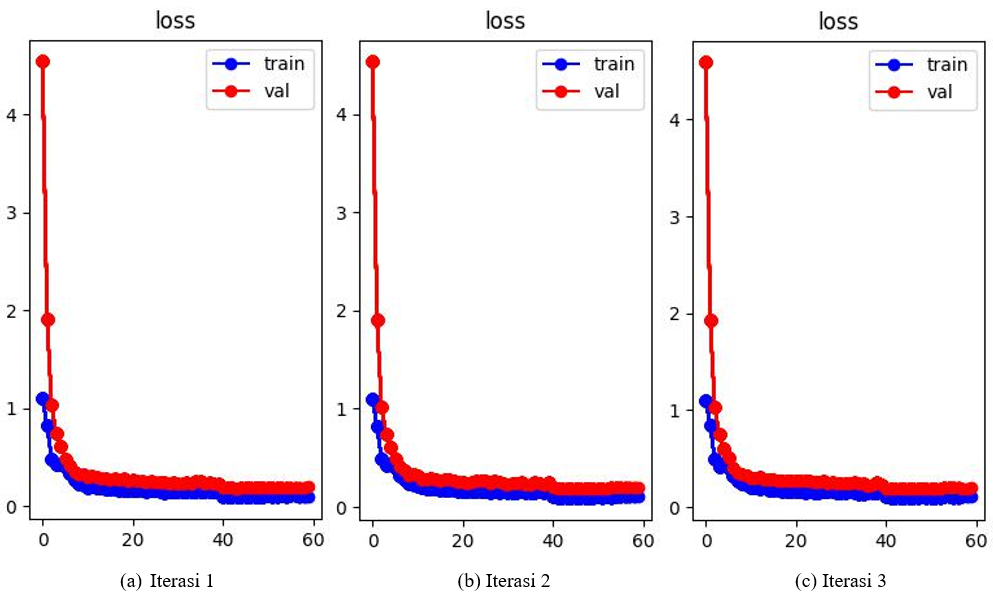
\includegraphics[scale=0.575]{gambar/Train SwinV2CP1 Loss.png}
  % Keterangan gambar yang diinputkan
  \caption{Grafik Loss Setiap Iterasi Swin Transformer V2 Parameter 2}
  % Label referensi dari gambar yang diinputkan
  \label{fig:grafiklossdariswinv2parameter2}
\end{figure}

\begin{figure}[ht]
  \centering
  % Nama dari file gambar yang diinputkan
  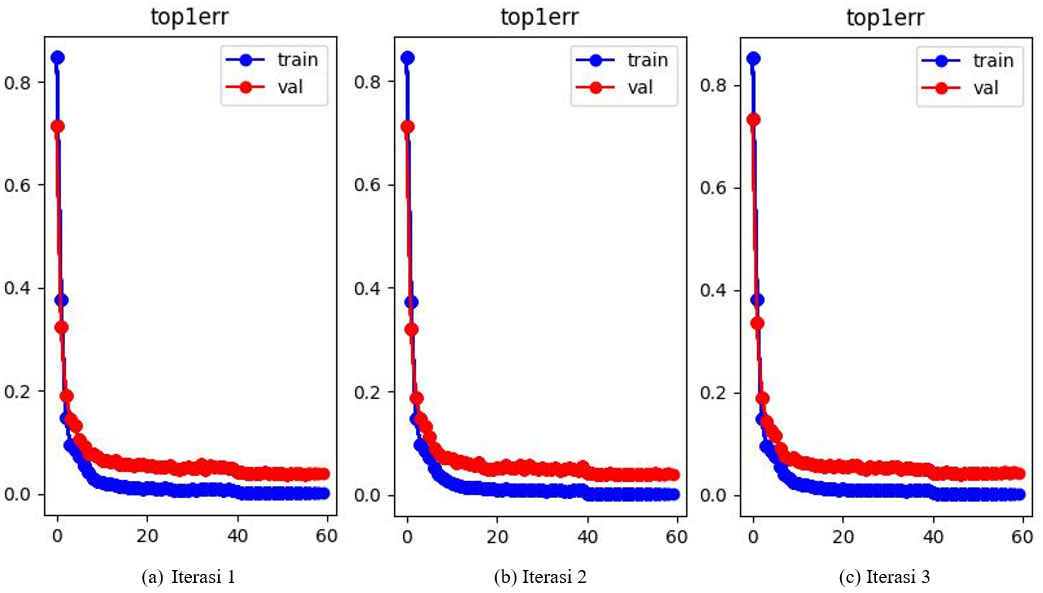
\includegraphics[scale=0.575]{gambar/Train SwinV2CP1 Top1Err.png}
  % Keterangan gambar yang diinputkan
  \caption{Grafik Top 1 Error Setiap Iterasi Swin Transformer V2 Parameter 2}
  % Label referensi dari gambar yang diinputkan
  \label{fig:grafiktop1errdariswinv2parameter2}
\end{figure}

Selain nilai akurasi, loss, dan Top 1 Error, diperoleh pula nilai mAP, rank@1, 
rank@5, rank@10 dari proses \emph{Testing} dan \emph{validation} pada 
masing-masing iterasi. Nilai tersebut dapat dilihat pada tabel 
\ref{tb:NilaimAP,Rank1,Rank5,danRank10ModelSwinTransformerV2Parameter2}.\\

% Selain gambar grafik diatas, diperoleh pula nilai mAP, rank@1, rank@5, rank@10 dari proses 
% \emph{Testing} pada masing-masing iterasi. Dari tiga kali iterasi tersebut, maka didapatkan 
% rata-rata dari model Swin Transformer V2 Parameter 2. Seluruh nilai iterasi dan rata-ratanya 
% dapat dilihat pada tabel 4.4.
% Diperoleh pula nilai mAP, rank@1, rank@5, rank@10 dari proses \emph{Testing} pada 
% masing-masing iterasi. Seluruh nilai tersebut dapat dilihat di tabel 4.2.

\begin{table}[h!]
  \begin{center}
  \caption{Nilai mAP, Rank@1, Rank@5, dan Rank@10 Swin Transformer V2 Parameter 2}
  \label{tb:NilaimAP,Rank1,Rank5,danRank10ModelSwinTransformerV2Parameter2}
  \begin{tabular}{|c|c|c|c|c|}
      \hline
      \textit{ } & \begin{tabular}[c]{@{}l@{}}\textbf{mAP}\end{tabular} & \begin{tabular}[c]{@{}l@{}}\textbf{Rank@1}\end{tabular} & \begin{tabular}[c]{@{}l@{}}\textbf{Rank@5}\end{tabular} & \begin{tabular}[c]{@{}l@{}}\textbf{Rank@10}\end{tabular}\\ \hline
      \textit{\textbf{Iterasi 1}} & \begin{tabular}[c]{@{}l@{}}0.752135\end{tabular} & \begin{tabular}[c]{@{}l@{}}\textbf{0.712202}\end{tabular} & \begin{tabular}[c]{@{}l@{}}\textbf{0.893988}\end{tabular} & \begin{tabular}[c]{@{}l@{}}0.930985\end{tabular}\\ \hline
      \textit{\textbf{Iterasi 2}} & \begin{tabular}[c]{@{}l@{}}0.752181\end{tabular} & \begin{tabular}[c]{@{}l@{}}0.711846\end{tabular} & \begin{tabular}[c]{@{}l@{}}0.891853\end{tabular} & \begin{tabular}[c]{@{}l@{}}0.927072\end{tabular}\\ \hline
      \textit{\textbf{Iterasi 3}} & \begin{tabular}[c]{@{}l@{}}\textbf{0.752636}\end{tabular} & \begin{tabular}[c]{@{}l@{}}\textbf{0.712202}\end{tabular} & \begin{tabular}[c]{@{}l@{}}0.892565\end{tabular} & \begin{tabular}[c]{@{}l@{}}\textbf{0.932764}\end{tabular}\\ \hline
      \textit{\textbf{Rata-Rata}} & \begin{tabular}[c]{@{}l@{}}0,751642\end{tabular} & \begin{tabular}[c]{@{}l@{}}0,712083\end{tabular} & \begin{tabular}[c]{@{}l@{}}0,892802\end{tabular} & \begin{tabular}[c]{@{}l@{}}0,930273\end{tabular}\\ \hline
  \end{tabular}
  \end{center}
\end{table}

\section{Analisa Hasil}
\label{sec:analisahasil}

% Dari tabel 4.1, tabel 4.2, serta grafik loss dan top 1 error yang ditampilkan pada bagian 4.1.1 dan 4.1.2, dapat diteliti 
% hasil model terbaik dari proses \emph{training} dan \emph{validation}. Iterasi dari masing-masing jenis model akan 
% mengambil hasil epoch terbaik dari proses \emph{training} dan \emph{validation}, sehingga hasil yang digunakan belum 
% tentu merupakan epoch terakhir dari proses \emph{training} dan \emph{validation}. Penjelasan terkait hasil dari setiap 
% jenis model yaitu sebagai berikut.

Dari seluruh data yang ditampilkan pada bagian 4.1, dapat diteliti hasil model terbaik dari proses \emph{training} dan 
\emph{validation}. Setiap jenis model re-identifikasi mobil akan mengambil hasil iterasi terbaik dari proses 
\emph{training} dan \emph{validation}. Penjelasan terkait hasil dari setiap jenis model yaitu sebagai berikut.

\subsection{Swin Transformer V1 Parameter 1}

Pada model Swin Transformer V1 parameter 1, model yang digunakan yaitu Swin-B (\emph{Base}), yang merupakan bentuk 
dasar dari arsitektur Swin Transformer. Dari tiga kali iterasi yang dilakukan, didapatkan data bahwa rata-rata nilai 
mAP (\emph{Mean Average Precision}) untuk model Swin Transformer V1 parameter 1 sebesar 0.668 atau 66.8\%. Dan untuk 
rank@1, rank@5, dan rank@10 berturut-turut sebesar 62.2\%, 82.6\%, dan 87\%. 

Berdasarkan Tabel \ref{tb:NilaimAP,Rank1,Rank5,danRank10ModelSwinTransformerV1Parameter1}, iterasi ketiga menjadi 
iterasi dengan hasil terbaik untuk model Swin Transformer V1 parameter 1. 
Hal ini didasarkan pada nilai mAP yang didapat yaitu sebesar 0.67 atau 67\%. Nilai tersebut 0.2\% lebih besar dari 
mAP rata-rata. Selain itu rank@1 yang didapat sebesar 62.3\% atau 0.1\% lebih besar dari rank@1 rata-rata. Rank@5 sebesar 
82.9\% atau 0.3\% lebih besar dari rank@5 rata-rata. Dan rank@10 sebesar 87.2\% atau 0.2\% lebih besar dari rank@10 
rata-rata.

\subsection{Swin Transformer V2 Parameter 1}

Pada model Swin Transformer V2 parameter 1, model yang digunakan yaitu Swin-B (\emph{Base}), yang merupakan bentuk 
dasar dari arsitektur Swin Transformer V2. Dari tiga kali iterasi yang dilakukan, didapatkan data bahwa rata-rata nilai 
mAP (\emph{Mean Average Precision}) untuk model Swin Transformer V2 parameter 1 sebesar 0.721 atau 72.1\%. Dan untuk 
rank@1, rank@5, dan rank@10 berturut-turut sebesar 68\%, 85.9\%, dan 90\%. 

Berdasarkan Tabel \Ref{tb:NilaimAP,Rank1,Rank5,danRank10ModelSwinTransformerV2Parameter1}, iterasi pertama menjadi 
iterasi dengan hasil terbaik untuk model Swin Transformer V2 parameter 1. 
Hal ini didasarkan pada nilai mAP yang didapat yaitu sebesar 0.725 atau 72.5\%. Nilai tersebut 0.4\% lebih besar dari 
mAP rata-rata. Selain itu rank@1 yang didapat sebesar 68.6\% atau 0.6\% lebih besar dari rank@1 rata-rata. Namun 
Rank@5 memiliki nilai sebesar 85.7\% atau 0.2\% lebih kecil dari rank@5 rata-rata. Dan rank@10 sebesar 89.5\% atau 0.5\% 
lebih kecil dari rank@10 rata-rata.

\subsection{Swin Transformer V1 Parameter 2}

Pada model Swin Transformer V1 parameter 2, model yang digunakan yaitu Swin-B (\emph{Base}), yang merupakan bentuk 
dasar dari arsitektur Swin Transformer. Dari tiga kali iterasi yang dilakukan, didapatkan data bahwa rata-rata nilai 
mAP (\emph{Mean Average Precision}) untuk model Swin Transformer V1 parameter 2 sebesar 0.746 atau 74.6\%. Dan untuk 
rank@1, rank@5, dan rank@10 berturut-turut sebesar 70.5\%, 88.8\%, dan 93\%. 

Berdasarkan Tabel \Ref{tb:NilaimAP,Rank1,Rank5,danRank10ModelSwinTransformerV1Parameter2}, iterasi kedua menjadi 
iterasi dengan hasil terbaik untuk model Swin Transformer V1 parameter 2. 
Hal ini didasarkan pada nilai mAP yang didapat yaitu sebesar 0.748 atau 74,8\%. Nilai tersebut 0.2\% lebih besar dari 
mAP rata-rata. Selain itu rank@1 yang didapat sebesar 70.6\% atau 0.1\% lebih besar dari rank@1 rata-rata. Rank@5 
memiliki nilai sebesar 89\% atau 0.2\% lebih besar dari rank@5 rata-rata. Namun rank@10 sebesar 93.2\% atau 0.2\% 
lebih kecil dari rank@10 rata-rata.

\subsection{Swin Transformer V2 Parameter 2}

Pada model Swin Transformer V2 parameter 2, model yang digunakan yaitu Swin-B (\emph{Base}), yang merupakan bentuk 
dasar dari arsitektur Swin Transformer V2. Dari tiga kali iterasi yang dilakukan, didapatkan data bahwa rata-rata nilai 
mAP (\emph{Mean Average Precision}) untuk model Swin Transformer V2 parameter 2 sebesar 0.751 atau 75.1\%. Dan untuk 
rank@1, rank@5, dan rank@10 berturut-turut sebesar 71.2\%, 89.2\%, dan 93\%. 

Berdasarkan Tabel \ref{tb:NilaimAP,Rank1,Rank5,danRank10ModelSwinTransformerV2Parameter2}, iterasi ketiga menjadi 
iterasi dengan hasil terbaik untuk model Swin Transformer V2 parameter 2. 
Hal ini didasarkan pada nilai mAP yang didapat yaitu sebesar 0.752 atau 75.2\%. Nilai tersebut 0.1\% lebih besar dari 
mAP rata-rata. Selain itu rank@1 yang didapat sebesar 71,2\% atau sama besar dengan rank@1 rata-rata. Rank@5 memiliki 
nilai sebesar 89.2\% atau sama besar dengan rank@5 rata-rata. Dan rank@10 sebesar 93.2\% atau 0.2\% 
lebih besar dari rank@10 rata-rata.

\section{Perbandingan Model Swin Transformer}
\label{sec:perbandinganmodelswintransformer}

Terdapat dua belas model yang telah dibuat pada penelitian ini, dengan setiap jenis modelnya dilakukan tiga kali iterasi. 
Perbandingan setiap jenis model beserta iterasinya dapat dilihat pada tabel 
\ref{tb:perbandingansetiapjenismodeldariswintransformer}. 

\begin{table}[h!]
  \begin{center}
  \caption{Perbandingan Setiap Jenis Model dari Swin Transformer }
  \label{tb:perbandingansetiapjenismodeldariswintransformer}
  \begin{tabular}{|c|c|c|c|c|c|}
      \hline
      \textbf{Jenis Model} & \begin{tabular}[c]{@{}l@{}}\textbf{Iterasi}\end{tabular} & \begin{tabular}[c]{@{}l@{}}\textbf{mAP}\end{tabular} & \begin{tabular}[c]{@{}l@{}}\textbf{Rank@1}\end{tabular} & \begin{tabular}[c]{@{}l@{}}\textbf{Rank@5}\end{tabular} & \begin{tabular}[c]{@{}l@{}}\textbf{Rank@10}\end{tabular}\\ \hline
      \multirow{3}{*}{\textbf{Swin T. V1 Parameter 1}} & \begin{tabular}[c]{@{}l@{}}Iterasi 1\end{tabular} & \begin{tabular}[c]{@{}l@{}}0.667091\end{tabular} & \begin{tabular}[c]{@{}l@{}}0.622199\end{tabular} & \begin{tabular}[c]{@{}l@{}}0.820704\end{tabular} & \begin{tabular}[c]{@{}l@{}}0.870153\end{tabular}\\
      & \begin{tabular}[c]{@{}l@{}}Iterasi 2\end{tabular} & \begin{tabular}[c]{@{}l@{}}0.667997\end{tabular} & \begin{tabular}[c]{@{}l@{}}0.621487\end{tabular} & \begin{tabular}[c]{@{}l@{}}0.827819\end{tabular} & \begin{tabular}[c]{@{}l@{}}0.869086\end{tabular}\\
      & \begin{tabular}[c]{@{}l@{}}Iterasi 3\end{tabular} & \begin{tabular}[c]{@{}l@{}}0.670210\end{tabular} & \begin{tabular}[c]{@{}l@{}}0.623621\end{tabular} & \begin{tabular}[c]{@{}l@{}}0.829598\end{tabular} & \begin{tabular}[c]{@{}l@{}}0.872643\end{tabular}\\ \hline
      \multirow{3}{*}{\textbf{Swin T. V2 Parameter 1}} & \begin{tabular}[c]{@{}l@{}}Iterasi 1\end{tabular} & \begin{tabular}[c]{@{}l@{}}0.725377\end{tabular} & \begin{tabular}[c]{@{}l@{}}0.686233\end{tabular} & \begin{tabular}[c]{@{}l@{}}0.857346\end{tabular} & \begin{tabular}[c]{@{}l@{}}0.895411\end{tabular}\\
      & \begin{tabular}[c]{@{}l@{}}Iterasi 2\end{tabular} & \begin{tabular}[c]{@{}l@{}}0.719978\end{tabular} & \begin{tabular}[c]{@{}l@{}}0.678762\end{tabular} & \begin{tabular}[c]{@{}l@{}}0.863750\end{tabular} & \begin{tabular}[c]{@{}l@{}}0.903949\end{tabular}\\
      & \begin{tabular}[c]{@{}l@{}}Iterasi 3\end{tabular} & \begin{tabular}[c]{@{}l@{}}0.717680\end{tabular} & \begin{tabular}[c]{@{}l@{}}0.676272\end{tabular} & \begin{tabular}[c]{@{}l@{}}0.857702\end{tabular} & \begin{tabular}[c]{@{}l@{}}0.900747\end{tabular}\\ \hline
      \multirow{3}{*}{\textbf{Swin T. V1 Parameter 2}} & \begin{tabular}[c]{@{}l@{}}Iterasi 1\end{tabular} & \begin{tabular}[c]{@{}l@{}}0.743027\end{tabular} & \begin{tabular}[c]{@{}l@{}}0.701530\end{tabular} & \begin{tabular}[c]{@{}l@{}}0.885094\end{tabular} & \begin{tabular}[c]{@{}l@{}}0.925294\end{tabular}\\
      & \begin{tabular}[c]{@{}l@{}}Iterasi 2\end{tabular} & \begin{tabular}[c]{@{}l@{}}0.748120\end{tabular} & \begin{tabular}[c]{@{}l@{}}0.706866\end{tabular} & \begin{tabular}[c]{@{}l@{}}0.890786\end{tabular} & \begin{tabular}[c]{@{}l@{}}0.932053\end{tabular}\\
      & \begin{tabular}[c]{@{}l@{}}Iterasi 3\end{tabular} & \begin{tabular}[c]{@{}l@{}}0.748066\end{tabular} & \begin{tabular}[c]{@{}l@{}}0.706510\end{tabular} & \begin{tabular}[c]{@{}l@{}}0.890430\end{tabular} & \begin{tabular}[c]{@{}l@{}}0.934543\end{tabular}\\ \hline
      \multirow{3}{*}{\textbf{Swin T. V2 Parameter 2}} & \begin{tabular}[c]{@{}l@{}}\textbf{Iterasi 1}\end{tabular} & \begin{tabular}[c]{@{}l@{}}0.752135\end{tabular} & \begin{tabular}[c]{@{}l@{}}\textbf{0.712202}\end{tabular} & \begin{tabular}[c]{@{}l@{}}\textbf{0.893988}\end{tabular} & \begin{tabular}[c]{@{}l@{}}\textbf{0.930985}\end{tabular}\\
      & \begin{tabular}[c]{@{}l@{}}Iterasi 2\end{tabular} & \begin{tabular}[c]{@{}l@{}}\textbf{0.752181}\end{tabular} & \begin{tabular}[c]{@{}l@{}}0.711846\end{tabular} & \begin{tabular}[c]{@{}l@{}}0.891853\end{tabular} & \begin{tabular}[c]{@{}l@{}}0.927072\end{tabular}\\
      & \begin{tabular}[c]{@{}l@{}}Iterasi 3\end{tabular} & \begin{tabular}[c]{@{}l@{}}0.751642\end{tabular} & \begin{tabular}[c]{@{}l@{}}0.712083\end{tabular} & \begin{tabular}[c]{@{}l@{}}0.892802\end{tabular} & \begin{tabular}[c]{@{}l@{}}0.930273\end{tabular}\\ \hline
    \end{tabular}
  \end{center}
\end{table}

Dari perbandingan tersebut dapat terlihat bahwa model Swin Transformer V2 parameter 2 pada iterasi pertama menjadi model 
dengan nilai rank@1, dan rank@5 tertinggi dari seluruh model yang telah dibuat serta memiliki selisih 
0.000046 dengan model yang memiliki mAP tertinggi yaitu Swin Transformer V2 parameter 2 iterasi kedua.

\section{Skenario Pengujian}
\label{sec:skenariopengujian}

Pengujian dilakukan menggunakan setiap jenis model re-identifikasi mobil yang telah dibuat pada penelitian ini. Setiap jenis model 
re-identifikasi mobil untuk pengujian hanya akan menggunakan salah satu dari tiga iterasi yang telah dibuat. Iterasi yang 
akan mewakili model re-identifikasi mobil ditentukan dari iterasi dengan nilai mAP dan rank@1 tertinggi yang didapat pada jenis 
model tersebut. Setiap model re-identifikasi mobil yang telah ditentukan akan melakukan pengujian menggunakan data kueri dan galeri 
yang telah tersedia dari dataset VRIC. Model re-identifikasi mobil yang digunakan untuk pengujian dapat dilihat pada 
tabel \ref{tb:modelreidentifikasiyangdigunakanpengujian}.

\begin{table}[h!]
  \begin{center}
  \caption{Model Re-Identifikasi yang Digunakan Pengujian}
  \label{tb:modelreidentifikasiyangdigunakanpengujian}
  \begin{tabular}{|c|c|c|c|}
      \hline
      \textbf{Jenis Model} & \begin{tabular}[c]{@{}l@{}}\textbf{Iterasi}\end{tabular} & \begin{tabular}[c]{@{}l@{}}\textbf{mAP}\end{tabular} & \begin{tabular}[c]{@{}l@{}}\textbf{Rank@1}\end{tabular}\\ \hline
      \begin{tabular}[c]{@{}l@{}}Swin T. V1 Parameter 1\end{tabular} & \begin{tabular}[c]{@{}l@{}}Iterasi 3\end{tabular} & \begin{tabular}[c]{@{}l@{}}0.670210\end{tabular} & \begin{tabular}[c]{@{}l@{}}0.623621\end{tabular}\\ \hline
      \begin{tabular}[c]{@{}l@{}}Swin T. V2 Parameter 1\end{tabular} & \begin{tabular}[c]{@{}l@{}}Iterasi 1\end{tabular} & \begin{tabular}[c]{@{}l@{}}0.725377\end{tabular} & \begin{tabular}[c]{@{}l@{}}0.686233\end{tabular}\\ \hline
      \begin{tabular}[c]{@{}l@{}}Swin T. V1 Parameter 2\end{tabular} & \begin{tabular}[c]{@{}l@{}}Iterasi 2\end{tabular} & \begin{tabular}[c]{@{}l@{}}0.748120\end{tabular} & \begin{tabular}[c]{@{}l@{}}0.706866\end{tabular}\\ \hline
      \begin{tabular}[c]{@{}l@{}}Swin T. V2 Parameter 2\end{tabular} & \begin{tabular}[c]{@{}l@{}}Iterasi 1\end{tabular} & \begin{tabular}[c]{@{}l@{}}0.752135\end{tabular} & \begin{tabular}[c]{@{}l@{}}0.712202\end{tabular}\\ \hline
  \end{tabular}
  \end{center}
\end{table}

Pengujian dilakukan dengan cara memasukkan sebuah citra kueri ke dalam model re-identifikasi. Model yang sudah memiliki 
galeri berisi kumpulan citra kemudian akan mencari citra dengan objek (mobil) di galeri yang memiliki kemiripan dengan citra 
kueri. Beberapa citra yang memiliki tingkat kemiripan tertinggi dengan kueri kemudian akan dibuat list peringkat 
kemiripan citra galeri berdasarkan citra kueri. Citra galeri yang memiliki objek yang sesuai dengan yang dicari dari citra 
kueri akan ditandai dengan warna hijau pada peringkatnya. Berikut merupakan beberapa hasil pengujian model re-identifikasi mobil.

\subsection{Pengujian Pertama}

Pengujian pertama menggunakan sebuah citra kueri ke-8 dengan objek minibus \linebreak berwarna krem dan putih. Citra kueri 
beserta hasil GradCAM dapat dilihat pada gambar \ref{fig:gambarkueriuntukpengujianpertama}.

\begin{figure}[h!]
  \centering
  \begin{subfigure}{.5\textwidth}
    \centering
    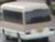
\includegraphics[width=.4\linewidth]{gambar/Que8_1018.jpg}
    \caption{Citra Kueri ke-8}
    \label{gambarkuerinomordelapan}
  \end{subfigure}%
  \begin{subfigure}{.5\textwidth}
    \centering
    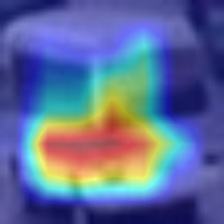
\includegraphics[width=.3\linewidth]{gambar/GradCamQue8_1018.jpg}
    \caption{GradCam Citra Kueri ke-8}
    \label{gradcamgambarkuerinomordelapan}
  \end{subfigure}
  \caption{Citra Kueri untuk Pengujian Pertama}
  \label{fig:gambarkueriuntukpengujianpertama}
\end{figure}

Citra galeri yang dicari pada pengujian pertama merupakan citra dengan objek \linebreak minibus yang sesuai dengan gambar 
\ref{fig:gambarkueriuntukpengujianpertama} dengan sudut pengambilan yang berbeda. Citra galeri beserta hasil GradCam dapat 
dilihat pada gambar \ref{fig:gambargaleriuntukpengujianpertama}.

\begin{figure}[h!]
  \centering
  \begin{subfigure}{.5\textwidth}
    \centering
    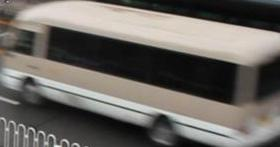
\includegraphics[width=.4\linewidth]{gambar/Gal8_1018.jpg}
    \caption{Citra Galeri yang Dicari}
    \label{gambargalerinomordelapan}
  \end{subfigure}%
  \begin{subfigure}{.5\textwidth}
    \centering
    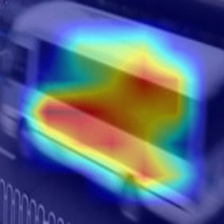
\includegraphics[width=.4\linewidth]{gambar/GradCamGal8_1018.jpg}
    \caption{GradCam Citra Galeri yang Dicari}
    \label{gradcamgambargalerinomordelapan}
  \end{subfigure}
  \caption{Citra Galeri yang Dicari untuk Pengujian Pertama}
  \label{fig:gambargaleriuntukpengujianpertama}
\end{figure}

Dengan memasukkan citra kueri ke-8 ke dalam model Swin Transformer V1 parameter 1 dengan iterasi 3, didapatkan hasil 
peringkat seperti yang terlihat pada gambar \ref{fig:hasilpengujianpertamapadamodelswintransformerv1param1}.

\begin{figure}[h!]
  \centering
  % Nama dari file gambar yang diinputkan
  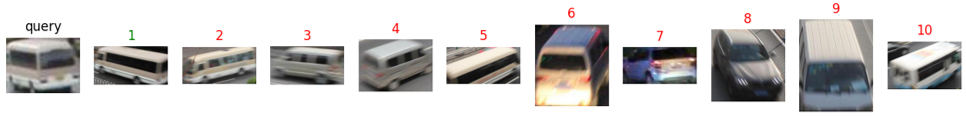
\includegraphics[scale=0.6]{gambar/Que8V1P1IT3.png}
  % Keterangan gambar yang diinputkan
  \caption{Hasil Pengujian Pertama pada Model Swin Transformer V1 Parameter 1}
  % Label referensi dari gambar yang diinputkan
  \label{fig:hasilpengujianpertamapadamodelswintransformerv1param1}
\end{figure}

Hasil pengujian yang didapat ketika memasukkan citra kueri ke-8 ke dalam model Swin Transformer V2 parameter 1 dengan 
iterasi 1 dapat dilihat pada gambar \ref{fig:hasilpengujianpertamapadamodelswintransformerv2param1}.

\begin{figure}[h!]
  \centering
  % Nama dari file gambar yang diinputkan
  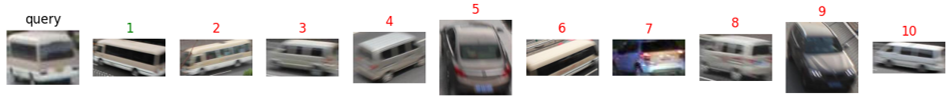
\includegraphics[scale=0.6]{gambar/Que8V2P1IT1.png}
  % Keterangan gambar yang diinputkan
  \caption{Hasil Pengujian Pertama pada Model Swin Transformer V2 Parameter 1}
  % Label referensi dari gambar yang diinputkan
  \label{fig:hasilpengujianpertamapadamodelswintransformerv2param1}
\end{figure}

Dari memasukkan citra kueri ke-8 ke dalam model Swin Transformer V1 parameter 2 dengan iterasi 2, didapatkan hasil 
peringkat yang dapat terlihat pada gambar \ref{fig:hasilpengujianpertamapadamodelswintransformerv1param2}.

\begin{figure}[h!]
  \centering
  % Nama dari file gambar yang diinputkan
  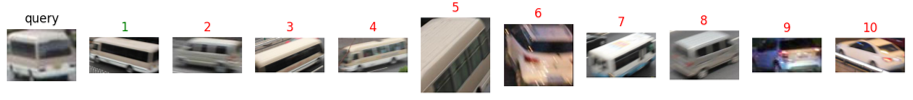
\includegraphics[scale=0.6]{gambar/Que8V1P2IT2.png}
  % Keterangan gambar yang diinputkan
  \caption{Hasil Pengujian Pertama pada Model Swin Transformer V1 Parameter 2}
  % Label referensi dari gambar yang diinputkan
  \label{fig:hasilpengujianpertamapadamodelswintransformerv1param2}
\end{figure}

Hasil pengujian dari model Swin Transformer V2 parameter 2 dengan iterasi 1 menggunakan citra kueri ke-8 dapat 
dilihat pada gambar \ref{fig:hasilpengujianpertamapadamodelswintransformerv2param2}.

\begin{figure}[h!]
  \centering
  % Nama dari file gambar yang diinputkan
  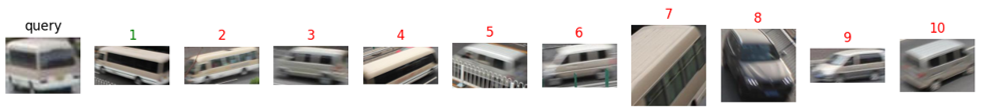
\includegraphics[scale=0.6]{gambar/Que8V2P2IT1.png}
  % Keterangan gambar yang diinputkan
  \caption{Hasil Pengujian Pertama pada Model Swin Transformer V2 Parameter 2}
  % Label referensi dari gambar yang diinputkan
  \label{fig:hasilpengujianpertamapadamodelswintransformerv2param2}
\end{figure}

Dari pengujian pertama, didapatkan hasil bahwa keempat model Swin Transformer yang berbeda dapat melakukan re-identifikasi 
dengan benar. Hal ini dibuktikan dengan ditunjukkannya citra galeri (gambar \ref{fig:gambargaleriuntukpengujianpertama})
berada pada peringkat pertama di hasil pengujian dari setiap model re-identifikasi.

\subsection{Pengujian Kedua}

Pengujian kedua menggunakan sebuah citra kueri ke-57 dengan objek mobil sedan berwarna biru tua yang terlihat dari samping 
dengan adanya blur. Citra kueri beserta hasil GradCam dapat dilihat pada gambar \ref{fig:gambarkueriuntukpengujiankedua}.

\begin{figure}[h!]
  \centering
  \begin{subfigure}{.5\textwidth}
    \centering
    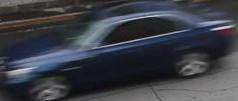
\includegraphics[width=.4\linewidth]{gambar/Que57_1112.jpg}
    \caption{Citra Kueri ke-57}
    \label{gambarkuerinomorlimatujuh}
  \end{subfigure}%
  \begin{subfigure}{.5\textwidth}
    \centering
    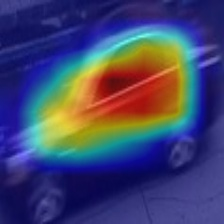
\includegraphics[width=.4\linewidth]{gambar/GradCamQue57_1112.jpg}
    \caption{GradCam Citra Kueri ke-57}
    \label{gradcamgambarkuerinomorlimatujuh}
  \end{subfigure}
  \caption{Citra Kueri untuk Pengujian Kedua}
  \label{fig:gambarkueriuntukpengujiankedua}
\end{figure}

Citra galeri yang dicari pada pengujian kedua merupakan citra dengan objek \linebreak mobil sedan berwarna biru tua 
yang sesuai dengan gambar \ref{fig:gambarkueriuntukpengujiankedua} dengan sudut pengambilan yang berbeda. Citra galeri 
beserta hasil GradCam dapat dilihat pada gambar \ref{fig:gambargaleriuntukpengujiankedua}.

\begin{figure}[h!]
  \centering
  \begin{subfigure}{.5\textwidth}
    \centering
    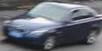
\includegraphics[width=.4\linewidth]{gambar/Gal57_1112.jpg}
    \caption{Citra Galeri yang Dicari}
    \label{gambargalerinomorlimatujuh}
  \end{subfigure}%
  \begin{subfigure}{.5\textwidth}
    \centering
    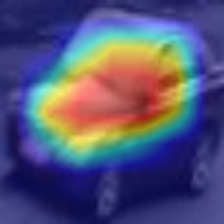
\includegraphics[width=.4\linewidth]{gambar/GradCamGal57_1112.jpg}
    \caption{GradCam Citra Galeri yang Dicari}
    \label{gradcamgambargalerinomorlimatujuh}
  \end{subfigure}
  \caption{Citra Galeri yang Dicari untuk Pengujian Kedua}
  \label{fig:gambargaleriuntukpengujiankedua}
\end{figure}

Hasil pengujian yang didapat ketika memasukkan citra kueri ke-57 ke dalam model Swin Transformer V1 parameter 1 dengan 
iterasi 3 dapat dilihat pada gambar \ref{fig:hasilpengujiankeduapadamodelswintransformerv1param1}.

\begin{figure}[h!]
  \centering
  % Nama dari file gambar yang diinputkan
  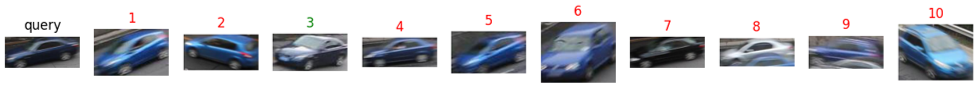
\includegraphics[scale=0.6]{gambar/qUE57v1P1IT3.png}
  % Keterangan gambar yang diinputkan
  \caption{Hasil Pengujian Kedua pada Model Swin Transformer V1 Parameter 1}
  % Label referensi dari gambar yang diinputkan
  \label{fig:hasilpengujiankeduapadamodelswintransformerv1param1}
\end{figure}

Dengan memasukkan citra kueri ke-57 ke dalam model Swin Transformer V2 parameter 1 dengan iterasi 1, didapatkan hasil 
peringkat seperti yang terlihat pada gambar \ref{fig:hasilpengujiankeduapadamodelswintransformerv2param1}.

\begin{figure}[h!]
  \centering
  % Nama dari file gambar yang diinputkan
  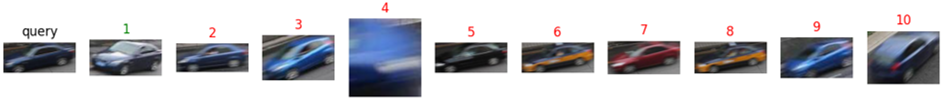
\includegraphics[scale=0.6]{gambar/Que57V2P1IT1.png}
  % Keterangan gambar yang diinputkan
  \caption{Hasil Pengujian Kedua pada Model Swin Transformer V2 Parameter 1}
  % Label referensi dari gambar yang diinputkan
  \label{fig:hasilpengujiankeduapadamodelswintransformerv2param1}
\end{figure}

Dari memasukkan citra kueri ke-57 ke dalam model Swin Transformer V1 parameter 2 dengan iterasi 2, didapatkan hasil 
peringkat yang dapat terlihat pada gambar \ref{fig:hasilpengujiankeduapadamodelswintransformerv1param2}.

\begin{figure}[h!]
  \centering
  % Nama dari file gambar yang diinputkan
  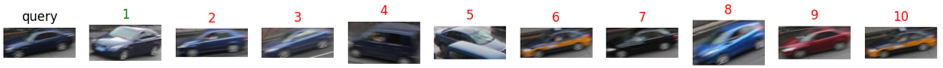
\includegraphics[scale=0.6]{gambar/Que57V1P2IT2.png}
  % Keterangan gambar yang diinputkan
  \caption{Hasil Pengujian Kedua pada Model Swin Transformer V1 Parameter 2}
  % Label referensi dari gambar yang diinputkan
  \label{fig:hasilpengujiankeduapadamodelswintransformerv1param2}
\end{figure}

Hasil pengujian dari model Swin Transformer V2 parameter 2 dengan iterasi 1 menggunakan gambar citra ke-57 dapat 
dilihat pada gambar \ref{fig:hasilpengujiankeduapadamodelswintransformerv2param2}.

\begin{figure}[h!]
  \centering
  % Nama dari file gambar yang diinputkan
  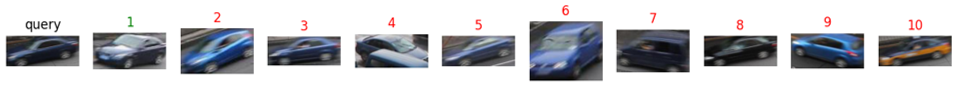
\includegraphics[scale=0.6]{gambar/Que57V2P2IT1.png}
  % Keterangan gambar yang diinputkan
  \caption{Hasil Pengujian Pertama pada Model Swin Transformer V2 Parameter 2}
  % Label referensi dari gambar yang diinputkan
  \label{fig:hasilpengujiankeduapadamodelswintransformerv2param2}
\end{figure}

Dari pengujian kedua, didapatkan hasil bahwa model Swin Transformer V1 parameter 1 gagal dalam melakukan re-identifikasi, 
karena citra kueri yang benar tidak berada pada peringkat pertama (gambar 
\ref{fig:hasilpengujiankeduapadamodelswintransformerv1param1}). Sementara ketiga model re-identifikasi lainnya berhasil 
melakukan re-identifikasi yang dibuktikan dengan ditunjukkannya citra galeri (gambar \ref{fig:gambargaleriuntukpengujianpertama})
berada pada peringkat pertama di hasil pengujian pada setiap model re-identifikasi.

\subsection{Pengujian Ketiga}

Pengujian ketiga menggunakan sebuah citra kueri ke-61 dengan objek mobil sedan berwarna putih. Citra kueri 
beserta hasil GradCam dapat dilihat pada gambar \ref{fig:gambarkueriuntukpengujianketiga}.

\begin{figure}[h!]
  \centering
  \begin{subfigure}{.5\textwidth}
    \centering
    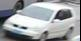
\includegraphics[width=.4\linewidth]{gambar/Que61_1120.jpg}
    \caption{Citra Kueri ke-61}
    \label{gambarkuerinomorenamsatu}
  \end{subfigure}%
  \begin{subfigure}{.5\textwidth}
    \centering
    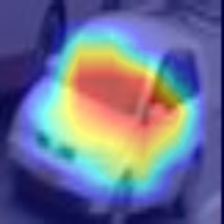
\includegraphics[width=.35\linewidth]{gambar/GradCamQue61_1120.jpg}
    \caption{GradCam Citra Kueri ke-61}
    \label{gradcamgambarkuerinomorenamsatu}
  \end{subfigure}
  \caption{Citra Kueri untuk Pengujian Ketiga}
  \label{fig:gambarkueriuntukpengujianketiga}
\end{figure}

Citra galeri yang dicari pada pengujian ketiga merupakan citra dengan objek mobil sedan berwarna putih 
yang sesuai dengan gambar \ref{fig:gambarkueriuntukpengujianketiga} dengan sudut pengambilan yang berbeda. 
Citra galeri beserta hasil GradCam dapat dilihat pada gambar \ref{fig:gambargaleriuntukpengujianketiga}.

\begin{figure}[h!]
  \centering
  \begin{subfigure}{.5\textwidth}
    \centering
    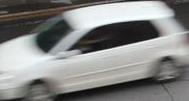
\includegraphics[width=.4\linewidth]{gambar/Gal61_1120.jpg}
    \caption{Citra Galeri yang Dicari}
    \label{gambargalerinomorenamsatu}
  \end{subfigure}%
  \begin{subfigure}{.5\textwidth}
    \centering
    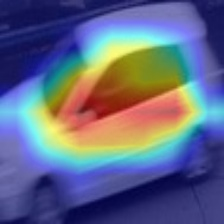
\includegraphics[width=.4\linewidth]{gambar/GradCamGal61_1120.jpg}
    \caption{GradCam Citra Galeri yang Dicari}
    \label{gradcamgambargalerinomorenamsatu}
  \end{subfigure}
  \caption{Citra Galeri yang Dicari untuk Pengujian Ketiga}
  \label{fig:gambargaleriuntukpengujianketiga}
\end{figure}

Dengan memasukkan citra kueri ke-61 ke dalam model Swin Transformer V1 parameter 1 dengan iterasi 3, didapatkan hasil 
peringkat seperti yang terlihat pada gambar \ref{fig:hasilpengujianketigapadamodelswintransformerv1param1}.

\begin{figure}[h!]
  \centering
  % Nama dari file gambar yang diinputkan
  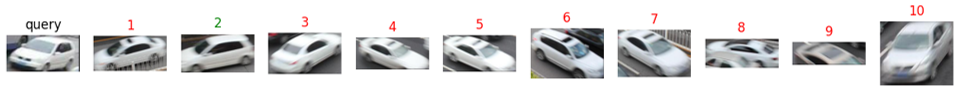
\includegraphics[scale=0.6]{gambar/Que61V1P1IT3.png}
  % Keterangan gambar yang diinputkan
  \caption{Hasil Pengujian Ketiga pada Model Swin Transformer V1 Parameter 1}
  % Label referensi dari gambar yang diinputkan
  \label{fig:hasilpengujianketigapadamodelswintransformerv1param1}
\end{figure}

Hasil pengujian yang didapat ketika memasukkan citra kueri ke-61 ke dalam model Swin Transformer V2 parameter 1 dengan 
iterasi 1 dapat dilihat pada gambar \ref{fig:hasilpengujianketigapadamodelswintransformerv2param1}.

\begin{figure}[h!]
  \centering
  % Nama dari file gambar yang diinputkan
  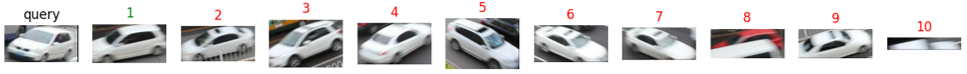
\includegraphics[scale=0.6]{gambar/Que61V2P1IT1.png}
  % Keterangan gambar yang diinputkan
  \caption{Hasil Pengujian Ketiga pada Model Swin Transformer V2 Parameter 1}
  % Label referensi dari gambar yang diinputkan
  \label{fig:hasilpengujianketigapadamodelswintransformerv2param1}
\end{figure}

Dari memasukkan citra kueri ke-61 ke dalam model Swin Transformer V1 parameter 2 dengan iterasi 2, didapatkan hasil 
peringkat yang dapat terlihat pada gambar \ref{fig:hasilpengujianketigapadamodelswintransformerv1param2}.

\begin{figure}[h!]
  \centering
  % Nama dari file gambar yang diinputkan
  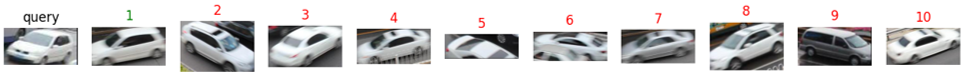
\includegraphics[scale=0.6]{gambar/Que61V1P2IT2.png}
  % Keterangan gambar yang diinputkan
  \caption{Hasil Pengujian Ketiga pada Model Swin Transformer V1 Parameter 2}
  % Label referensi dari gambar yang diinputkan
  \label{fig:hasilpengujianketigapadamodelswintransformerv1param2}
\end{figure}

Hasil pengujian dari model Swin Transformer V2 parameter 2 dengan iterasi 1 menggunakan citra kueri ke-61 dapat 
dilihat pada gambar \ref{fig:hasilpengujianketigapadamodelswintransformerv2param2}.

\begin{figure}[h!]
  \centering
  % Nama dari file gambar yang diinputkan
  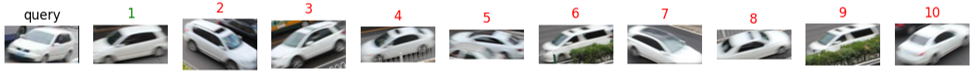
\includegraphics[scale=0.6]{gambar/Que61V2P2IT1.png}
  % Keterangan gambar yang diinputkan
  \caption{Hasil Pengujian Ketiga pada Model Swin Transformer V2 Parameter 2}
  % Label referensi dari gambar yang diinputkan
  \label{fig:hasilpengujianketigapadamodelswintransformerv2param2}
\end{figure}

Dari pengujian ketiga, didapatkan hasil bahwa model Swin Transformer V1 parameter 1 gagal dalam melakukan re-identifikasi, 
karena citra kueri yang benar tidak berada pada peringkat pertama (gambar 
\ref{fig:hasilpengujianketigapadamodelswintransformerv1param1}). Sementara ketiga model re-identifikasi lainnya berhasil 
melakukan re-identifikasi. Hal ini dibuktikan dengan ditunjukkannya citra galeri (gambar \ref{fig:gambargaleriuntukpengujianketiga})
berada pada peringkat pertama di hasil pengujian pada setiap model re-identifikasi.

\subsection{Pengujian Keempat}

Pengujian keempat menggunakan sebuah citra kueri ke-21 dengan objek mobil sedan berwarna merah. Citra kueri 
beserta hasil GradCam dapat dilihat pada gambar \ref{fig:gambarkueriuntukpengujiankeempat}.

\begin{figure}[h!]
  \centering
  \begin{subfigure}{.5\textwidth}
    \centering
    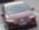
\includegraphics[width=.4\linewidth]{gambar/Que21_1046.jpg}
    \caption{Citra Kueri ke-21}
    \label{gambarkuerinomorduasatu}
  \end{subfigure}%
  \begin{subfigure}{.5\textwidth}
    \centering
    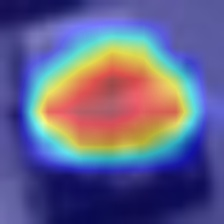
\includegraphics[width=.4\linewidth]{gambar/GradCamQue21_1046.jpg}
    \caption{GradCam Citra Kueri ke-21}
    \label{gradcamgambarkuerinomorduasatu}
  \end{subfigure}
  \caption{Citra Kueri untuk Pengujian Keempat}
  \label{fig:gambarkueriuntukpengujiankeempat}
\end{figure}

Citra galeri yang dicari pada pengujian keempat merupakan citra dengan objek \linebreak mobil sedan berwarna merah 
yang sesuai dengan gambar \ref{fig:gambarkueriuntukpengujiankeempat} dengan sudut pengambilan yang berbeda. 
Citra galeri beserta hasil GradCam dapat dilihat pada gambar \ref{fig:gambargaleriuntukpengujiankeempat}.\\

\begin{figure}[h!]
  \centering
  \begin{subfigure}{.5\textwidth}
    \centering
    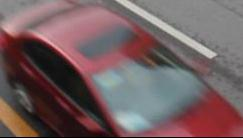
\includegraphics[width=.4\linewidth]{gambar/Gal21_1046.jpg}
    \caption{Citra Galeri yang Dicari}
    \label{gambargalerinomorduasatu}
  \end{subfigure}%
  \begin{subfigure}{.5\textwidth}
    \centering
    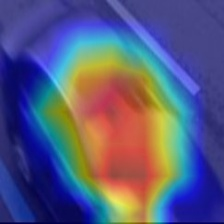
\includegraphics[width=.4\linewidth]{gambar/GradCamGal21_1046.jpg}
    \caption{GradCam Citra Galeri yang Dicari}
    \label{gradcamgambargalerinomorduasatu}
  \end{subfigure}
  \caption{Citra Galeri yang Dicari untuk Pengujian Keempat}
  \label{fig:gambargaleriuntukpengujiankeempat}
\end{figure}

Dengan memasukkan citra kueri ke-21 ke dalam model Swin Transformer V1 parameter 1 dengan iterasi 3, didapatkan hasil 
peringkat seperti yang terlihat pada gambar \ref{fig:hasilpengujiankeempatpadamodelswintransformerv1param1}.

\begin{figure}[h!]
  \centering
  % Nama dari file gambar yang diinputkan
  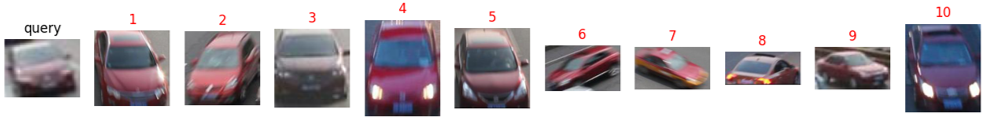
\includegraphics[scale=0.6]{gambar/Que21V1P1IT3.png}
  % Keterangan gambar yang diinputkan
  \caption{Hasil Pengujian Keempat pada Model Swin Transformer V1 Parameter 1}
  % Label referensi dari gambar yang diinputkan
  \label{fig:hasilpengujiankeempatpadamodelswintransformerv1param1}
\end{figure}

Hasil pengujian yang didapat ketika memasukkan citra kueri ke-21 ke dalam model Swin Transformer V2 parameter 1 dengan 
iterasi 1 dapat dilihat pada gambar \ref{fig:hasilpengujiankeempatpadamodelswintransformerv2param1}.

\begin{figure}[h!]
  \centering
  % Nama dari file gambar yang diinputkan
  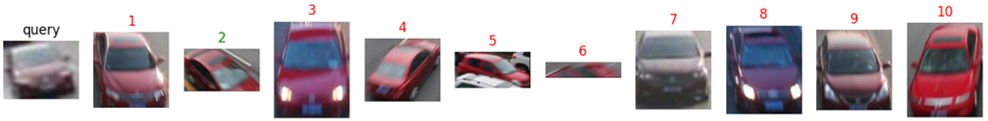
\includegraphics[scale=0.6]{gambar/Que21V2P1IT1.png}
  % Keterangan gambar yang diinputkan
  \caption{Hasil Pengujian Keempat pada Model Swin Transformer V2 Parameter 1}
  % Label referensi dari gambar yang diinputkan
  \label{fig:hasilpengujiankeempatpadamodelswintransformerv2param1}
\end{figure}

Dari memasukkan citra kueri ke-21 ke dalam model Swin Transformer V1 parameter 2 dengan iterasi 2, didapatkan hasil 
peringkat yang dapat terlihat pada gambar \ref{fig:hasilpengujiankeempatpadamodelswintransformerv1param2}.

\begin{figure}[h!]
  \centering
  % Nama dari file gambar yang diinputkan
  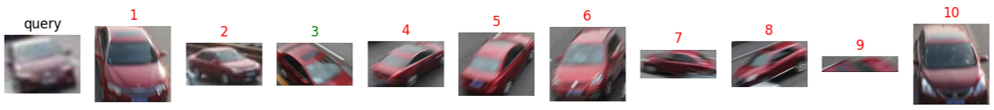
\includegraphics[scale=0.6]{gambar/Que21V1P2IT2.png}
  % Keterangan gambar yang diinputkan
  \caption{Hasil Pengujian Keempat pada Model Swin Transformer V1 Parameter 2}
  % Label referensi dari gambar yang diinputkan
  \label{fig:hasilpengujiankeempatpadamodelswintransformerv1param2}
\end{figure}

Hasil pengujian dari model Swin Transformer V2 parameter 2 dengan iterasi 1 menggunakan citra kueri ke-21 dapat 
dilihat pada gambar \ref{fig:hasilpengujiankeempatpadamodelswintransformerv2param2}.

\begin{figure}[h!]
  \centering
  % Nama dari file gambar yang diinputkan
  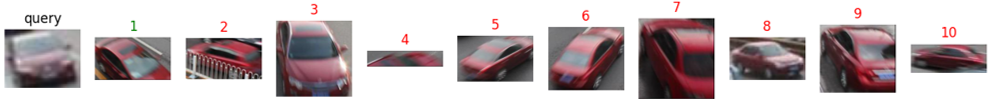
\includegraphics[scale=0.6]{gambar/Que21V2P2IT1.png}
  % Keterangan gambar yang diinputkan
  \caption{Hasil Pengujian Keempat pada Model Swin Transformer V2 Parameter 2}
  % Label referensi dari gambar yang diinputkan
  \label{fig:hasilpengujiankeempatpadamodelswintransformerv2param2}
\end{figure}

Dari pengujian keempat, didapatkan hasil bahwa model Swin Transformer V1 parameter 1 gagal dalam melakukan re-identifikasi, 
karena citra kueri yang benar tidak berada pada sepuluh peringkat teratas (gambar 
\ref{fig:hasilpengujiankeempatpadamodelswintransformerv1param1}). Sementara model Swin Transformer V2 parameter 1 dan 
Swin Transformer V1 parameter 2 masih dapat melakukan re-identifikasi sesuai citra kueri, namun citra galeri yang tepat 
tidak berada pada peringkat pertama (seperti yang terlihat pada gambar \ref{fig:hasilpengujiankeempatpadamodelswintransformerv2param1} 
dan gambar \ref{fig:hasilpengujiankeempatpadamodelswintransformerv1param2}). Model Swin Transformer V2 parameter 2 berhasil 
melakukan re-identifikasi pada pengujian keempat. Hal ini dibuktikan dengan ditunjukkannya citra galeri 
(gambar \ref{fig:gambargaleriuntukpengujiankeempat}) berada pada peringkat pertama di hasil pengujian model Swin Transformer 
V2 parameter 2 (gambar \ref{fig:hasilpengujiankeempatpadamodelswintransformerv2param2}).

\subsection{Pengujian Kelima}

Pengujian kelima menggunakan sebuah citra kueri ke-9 dengan objek mobil suv berwarna hitam. Citra kueri 
beserta hasil GradCam dapat dilihat pada gambar \ref{fig:gambarkueriuntukpengujiankelima}.

\begin{figure}[h!]
  \centering
  \begin{subfigure}{.5\textwidth}
    \centering
    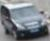
\includegraphics[width=.4\linewidth]{gambar/Que9_1019.jpg}
    \caption{Citra Kueri ke-9}
    \label{gambarkuerinomorsembilan}
  \end{subfigure}%
  \begin{subfigure}{.5\textwidth}
    \centering
    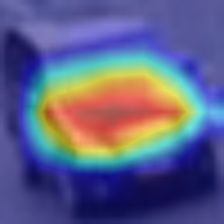
\includegraphics[width=.4\linewidth]{gambar/GradCamQue9_1019.jpg}
    \caption{GradCam Citra Kueri ke-9}
    \label{gradcamgambarkuerinomorsembilan}
  \end{subfigure}
  \caption{Citra Kueri untuk Pengujian Kelima}
  \label{fig:gambarkueriuntukpengujiankelima}
\end{figure}

Citra galeri yang dicari pada pengujian kelima merupakan citra dengan objek \linebreak mobil suv berwarna hitam 
yang sesuai dengan gambar \ref{fig:gambarkueriuntukpengujiankelima} dengan sudut pengambilan yang berbeda. 
Citra galeri beserta hasil GradCam dapat dilihat pada gambar \ref{fig:gambargaleriuntukpengujiankelima}.

\begin{figure}[h!]
  \centering
  \begin{subfigure}{.5\textwidth}
    \centering
    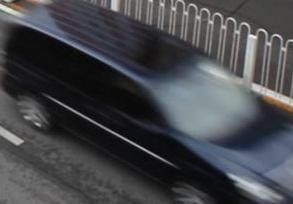
\includegraphics[width=.4\linewidth]{gambar/Gal9_1019.jpg}
    \caption{Citra Galeri yang Dicari}
    \label{gambargalerinomorsembilan}
  \end{subfigure}%
  \begin{subfigure}{.5\textwidth}
    \centering
    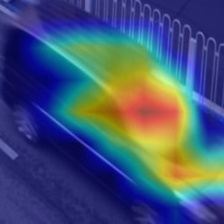
\includegraphics[width=.4\linewidth]{gambar/GradCamGal9_1019.jpg}
    \caption{GradCam Citra Galeri yang Dicari}
    \label{gradcamgambargalerinomorsembilan}
  \end{subfigure}
  \caption{Citra Galeri yang Dicari untuk Pengujian Kelima}
  \label{fig:gambargaleriuntukpengujiankelima}
\end{figure}

Dengan memasukkan citra kueri ke-9 ke dalam model Swin Transformer V1 parameter 1 dengan iterasi 3, didapatkan hasil 
peringkat seperti yang terlihat pada gambar \ref{fig:hasilpengujiankelimapadamodelswintransformerv1param1}.

\begin{figure}[h!]
  \centering
  % Nama dari file gambar yang diinputkan
  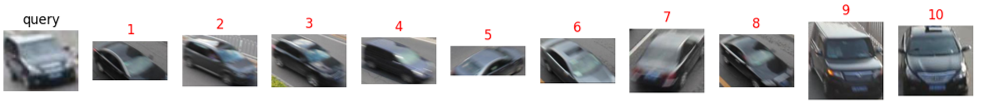
\includegraphics[scale=0.6]{gambar/Que9V1P1IT3.png}
  % Keterangan gambar yang diinputkan
  \caption{Hasil Pengujian Kelima pada Model Swin Transformer V1 Parameter 1}
  % Label referensi dari gambar yang diinputkan
  \label{fig:hasilpengujiankelimapadamodelswintransformerv1param1}
\end{figure}

Hasil pengujian yang didapat ketika memasukkan citra kueri ke-9 ke dalam model Swin Transformer V2 parameter 1 dengan 
iterasi 1 dapat dilihat pada gambar \ref{fig:hasilpengujiankelimapadamodelswintransformerv2param1}.

\begin{figure}[h!]
  \centering
  % Nama dari file gambar yang diinputkan
  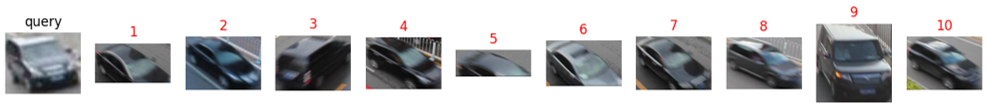
\includegraphics[scale=0.6]{gambar/Que9V2P1IT1.png}
  % Keterangan gambar yang diinputkan
  \caption{Hasil Pengujian Kelima pada Model Swin Transformer V2 Parameter 1}
  % Label referensi dari gambar yang diinputkan
  \label{fig:hasilpengujiankelimapadamodelswintransformerv2param1}
\end{figure}

Dari memasukkan citra kueri ke-9 ke dalam model Swin Transformer V1 parameter 2 dengan iterasi 2, didapatkan hasil 
peringkat yang dapat terlihat pada gambar \ref{fig:hasilpengujiankelimapadamodelswintransformerv1param2}.

\begin{figure}[h!]
  \centering
  % Nama dari file gambar yang diinputkan
  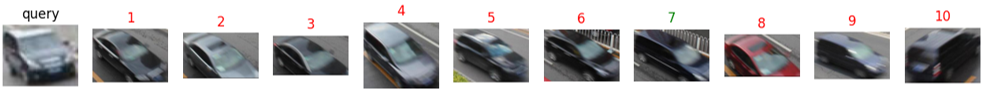
\includegraphics[scale=0.6]{gambar/Que9V1P2IT2.png}
  % Keterangan gambar yang diinputkan
  \caption{Hasil Pengujian Kelima pada Model Swin Transformer V1 Parameter 2}
  % Label referensi dari gambar yang diinputkan
  \label{fig:hasilpengujiankelimapadamodelswintransformerv1param2}
\end{figure}

Hasil pengujian dari model Swin Transformer V2 parameter 2 dengan iterasi 1 menggunakan citra kueri ke-9 dapat 
dilihat pada gambar \ref{fig:hasilpengujiankelimapadamodelswintransformerv2param2}.

\begin{figure}[h!]
  \centering
  % Nama dari file gambar yang diinputkan
  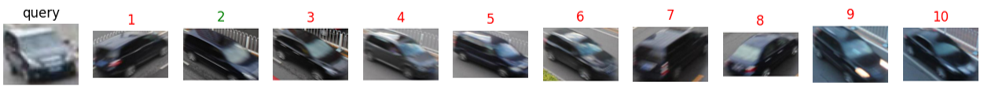
\includegraphics[scale=0.6]{gambar/Que9V2P2IT1.png}
  % Keterangan gambar yang diinputkan
  \caption{Hasil Pengujian Kelima pada Model Swin Transformer V2 Parameter 2}
  % Label referensi dari gambar yang diinputkan
  \label{fig:hasilpengujiankelimapadamodelswintransformerv2param2}
\end{figure}

Dari pengujian kelima, didapatkan hasil bahwa Swin Transformer V1 parameter 1 dan Swin Transformer V2 parameter 1 
gagal dalam melakukan re-identifikasi, karena citra kueri yang benar tidak berada di sepuluh peringkat teratas (gambar 
\ref{fig:hasilpengujiankelimapadamodelswintransformerv1param1} dan gambar 
\ref{fig:hasilpengujiankelimapadamodelswintransformerv2param1}). Sementara pada Swin Transformer V1 parameter 2, citra 
galeri hanya berada pada peringkat ke-7 (gambar \ref{fig:hasilpengujiankelimapadamodelswintransformerv1param2}). 
Dan untuk Swin Transformer V2 parameter 2, dapat melakukan 
re-identifikasi namun citra galeri hanya berada pada peringkat ke-2 seperti yang terlihat pada gambar 
\ref{fig:hasilpengujiankelimapadamodelswintransformerv2param2}.

\subsection{Pengujian Keenam}

Pengujian keenam menggunakan sebuah citra kueri ke-29 dengan objek mobil taksi \linebreak berwarna biru tua dan oranye, dengan sebagian 
badan mobil tertutup oleh objek lain. Citra kueri beserta hasil GradCam dapat dilihat pada gambar 
\ref{fig:gambarkueriuntukpengujiankeenam}.

\begin{figure}[h!]
  \centering
  \begin{subfigure}{.5\textwidth}
    \centering
    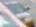
\includegraphics[width=.4\linewidth]{gambar/Que29_1060.jpg}
    \caption{Citra Kueri ke-29}
    \label{gambarkuerinomorduasembilan}
  \end{subfigure}%
  \begin{subfigure}{.5\textwidth}
    \centering
    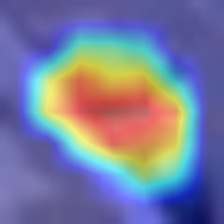
\includegraphics[width=.4\linewidth]{gambar/GradCamQue29_1060.jpg}
    \caption{GradCam Citra Kueri ke-29}
    \label{gradcamgambarkuerinomorduasembilan}
  \end{subfigure}
  \caption{Citra Kueri untuk Pengujian Keenam}
  \label{fig:gambarkueriuntukpengujiankeenam}
\end{figure}

Citra galeri yang dicari pada pengujian keenam merupakan citra dengan objek mobil taksi berwarna biru tua 
dan oranye yang sesuai dengan gambar \ref{fig:gambarkueriuntukpengujiankeenam} dengan sudut pengambilan yang berbeda. 
Citra galeri beserta hasil GradCam dapat dilihat pada gambar \ref{fig:gambargaleriuntukpengujiankeenam}.

\begin{figure}[h!]
  \centering
  \begin{subfigure}{.5\textwidth}
    \centering
    \includegraphics[width=.4\linewidth]{gambar/Gal29_1060.jpg}
    \caption{Citra Galeri yang Dicari}
    \label{gambargalerinomorduasembilan}
  \end{subfigure}%
  \begin{subfigure}{.5\textwidth}
    \centering
    \includegraphics[width=.4\linewidth]{gambar/GradCamGal29_1060.jpg}
    \caption{GradCam Citra Galeri yang Dicari}
    \label{gradcamgambargalerinomorduasembilan}
  \end{subfigure}
  \caption{Citra Galeri yang Dicari untuk Pengujian Keenam}
  \label{fig:gambargaleriuntukpengujiankeenam}
\end{figure}

Dengan memasukkan citra kueri ke-29 ke dalam model Swin Transformer V1 parameter 1 dengan iterasi 3, didapatkan hasil 
peringkat seperti yang terlihat pada gambar \ref{fig:hasilpengujiankeenampadamodelswintransformerv1param1}.

\begin{figure}[h!]
  \centering
  % Nama dari file gambar yang diinputkan
  \includegraphics[scale=0.6]{gambar/Que29V1P1IT3.png}
  % Keterangan gambar yang diinputkan
  \caption{Hasil Pengujian Keenam pada Model Swin Transformer V1 Parameter 1}
  % Label referensi dari gambar yang diinputkan
  \label{fig:hasilpengujiankeenampadamodelswintransformerv1param1}
\end{figure}

Hasil pengujian yang didapat ketika memasukkan citra kueri ke-29 ke dalam model Swin Transformer V2 parameter 1 dengan 
iterasi 1 dapat dilihat pada gambar \ref{fig:hasilpengujiankeenampadamodelswintransformerv2param1}.

\begin{figure}[h!]
  \centering
  % Nama dari file gambar yang diinputkan
  \includegraphics[scale=0.6]{gambar/Que29V2P1IT1.png}
  % Keterangan gambar yang diinputkan
  \caption{Hasil Pengujian Keenam pada Model Swin Transformer V2 Parameter 1}
  % Label referensi dari gambar yang diinputkan
  \label{fig:hasilpengujiankeenampadamodelswintransformerv2param1}
\end{figure}

Dari memasukkan citra kueri ke-29 ke dalam model Swin Transformer V1 parameter 2 dengan iterasi 2, didapatkan hasil 
peringkat yang dapat terlihat pada gambar \ref{fig:hasilpengujiankeenampadamodelswintransformerv1param2}.

\begin{figure}[h!]
  \centering
  % Nama dari file gambar yang diinputkan
  \includegraphics[scale=0.6]{gambar/Que29V1P2IT2.png}
  % Keterangan gambar yang diinputkan
  \caption{Hasil Pengujian Keenam pada Model Swin Transformer V1 Parameter 2}
  % Label referensi dari gambar yang diinputkan
  \label{fig:hasilpengujiankeenampadamodelswintransformerv1param2}
\end{figure}

Hasil pengujian dari model Swin Transformer V2 parameter 2 dengan iterasi 1 menggunakan citra kueri ke-29 dapat 
dilihat pada gambar \ref{fig:hasilpengujiankeenampadamodelswintransformerv2param2}.

\begin{figure}[h!]
  \centering
  % Nama dari file gambar yang diinputkan
  \includegraphics[scale=0.6]{gambar/Que29V2P2IT1.png}
  % Keterangan gambar yang diinputkan
  \caption{Hasil Pengujian Keenam pada Model Swin Transformer V2 Parameter 2}
  % Label referensi dari gambar yang diinputkan
  \label{fig:hasilpengujiankeenampadamodelswintransformerv2param2}
\end{figure}

Dari pengujian keenam, didapatkan hasil bahwa seluruh model Swin Transformer pada penelitian ini tidak mampu dalam melakukan 
re-identifikasi ketika diberikan citra yang objeknya tertimpa oleh objek lain. Hal ini dapat dilihat dari hasil peringkat 
sepuluh teratas dari setiap model tidak menunjukan adanya citra galeri (gambar \ref{fig:gambargaleriuntukpengujiankeenam}) 
pada daftar peringkat yang ada. Hasil pengujian ini memperlihatkan bahwa jika citra kueri dengan objek yang setengah utuh 
ingin diidentifikasi ulang, model re-identifikasi kesulitan untuk mengenali objek tersebut.

\subsection{Pengujian Ketujuh}

Pengujian ketujuh menggunakan sebuah citra kueri ke-70 dengan objek mobil suv \linebreak berwarna hitam. Citra kueri 
beserta hasil GradCam dapat dilihat pada gambar \ref{fig:gambarkueriuntukpengujianketujuh}.

\begin{figure}[h!]
  \centering
  \begin{subfigure}{.5\textwidth}
    \centering
    \includegraphics[width=.4\linewidth]{gambar/Que70_114.jpg}
    \caption{Citra Kueri ke-70}
    \label{gambarkuerinomortujuhpuluh}
  \end{subfigure}%
  \begin{subfigure}{.5\textwidth}
    \centering
    \includegraphics[width=.4\linewidth]{gambar/GradCamQue70_114.jpg}
    \caption{GradCam Citra Kueri ke-70}
    \label{gradcamgambarkuerinomortujuhpuluh}
  \end{subfigure}
  \caption{Citra Kueri untuk Pengujian Ketujuh}
  \label{fig:gambarkueriuntukpengujianketujuh}
\end{figure}

Citra galeri yang dicari pada pengujian ketujuh merupakan citra dengan objek mobil suv berwarna hitam 
yang sesuai dengan gambar \ref{fig:gambarkueriuntukpengujianketujuh} dengan sudut pengambilan yang berbeda. 
Citra galeri beserta hasil GradCam dapat dilihat pada gambar \ref{fig:gambargaleriuntukpengujianketujuh}.

\begin{figure}[h!]
  \centering
  \begin{subfigure}{.5\textwidth}
    \centering
    \includegraphics[width=.4\linewidth]{gambar/Gal70_114.jpg}
    \caption{Citra Galeri yang Dicari}
    \label{gambargalerinomortujuhpuluh}
  \end{subfigure}%
  \begin{subfigure}{.5\textwidth}
    \centering
    \includegraphics[width=.4\linewidth]{gambar/GradCamGal70_114.jpg}
    \caption{GradCam Citra Galeri yang Dicari}
    \label{gradcamgambargalerinomortujuhpuluh}
  \end{subfigure}
  \caption{Citra Galeri yang Dicari untuk Pengujian Ketujuh}
  \label{fig:gambargaleriuntukpengujianketujuh}
\end{figure}

Dengan memasukkan citra kueri ke-70 ke dalam model Swin Transformer V1 parameter 1 dengan iterasi 3, didapatkan hasil 
peringkat seperti yang terlihat pada gambar \ref{fig:hasilpengujianketujuhpadamodelswintransformerv1param1}.

\begin{figure}[h!]
  \centering
  % Nama dari file gambar yang diinputkan
  \includegraphics[scale=0.6]{gambar/Que70V1P1IT3.png}
  % Keterangan gambar yang diinputkan
  \caption{Hasil Pengujian Ketujuh pada Model Swin Transformer V1 Parameter 1}
  % Label referensi dari gambar yang diinputkan
  \label{fig:hasilpengujianketujuhpadamodelswintransformerv1param1}
\end{figure}

Hasil pengujian yang didapat ketika memasukkan citra kueri ke-70 ke dalam model Swin Transformer V2 parameter 1 dengan 
iterasi 1 dapat dilihat pada gambar \ref{fig:hasilpengujianketujuhpadamodelswintransformerv2param1}.

\begin{figure}[h!]
  \centering
  % Nama dari file gambar yang diinputkan
  \includegraphics[scale=0.6]{gambar/Que70V2P1IT1.png}
  % Keterangan gambar yang diinputkan
  \caption{Hasil Pengujian Ketujuh pada Model Swin Transformer V2 Parameter 1}
  % Label referensi dari gambar yang diinputkan
  \label{fig:hasilpengujianketujuhpadamodelswintransformerv2param1}
\end{figure}

Dari memasukkan citra kueri ke-70 ke dalam model Swin Transformer V1 parameter 2 dengan iterasi 2, didapatkan hasil 
peringkat yang dapat terlihat pada gambar \ref{fig:hasilpengujianketujuhpadamodelswintransformerv1param2}.

\begin{figure}[h!]
  \centering
  % Nama dari file gambar yang diinputkan
  \includegraphics[scale=0.6]{gambar/Que70V1P2IT2.png}
  % Keterangan gambar yang diinputkan
  \caption{Hasil Pengujian Ketujuh pada Model Swin Transformer V1 Parameter 2}
  % Label referensi dari gambar yang diinputkan
  \label{fig:hasilpengujianketujuhpadamodelswintransformerv1param2}
\end{figure}

Hasil pengujian dari model Swin Transformer V2 parameter 2 dengan iterasi 1 menggunakan citra kueri ke-70 dapat 
dilihat pada gambar \ref{fig:hasilpengujianketujuhpadamodelswintransformerv2param2}.

\begin{figure}[h!]
  \centering
  % Nama dari file gambar yang diinputkan
  \includegraphics[scale=0.6]{gambar/Que70V2P2IT1.png}
  % Keterangan gambar yang diinputkan
  \caption{Hasil Pengujian Ketujuh pada Model Swin Transformer V2 Parameter 2}
  % Label referensi dari gambar yang diinputkan
  \label{fig:hasilpengujianketujuhpadamodelswintransformerv2param2}
\end{figure}

Dari pengujian ketujuh, didapatkan hasil bahwa seluruh model Swin Transformer pada penelitian ini tidak mampu dalam melakukan 
re-identifikasi ketika diberikan citra kueri ke-70. Hal ini dapat dilihat dari hasil peringkat sepuluh teratas dari setiap 
model tidak menunjukan adanya citra galeri (gambar \ref{fig:gambargaleriuntukpengujianketujuh}) pada daftar peringkat yang 
ada. Hasil pengujian ini memperlihatkan bahwa jika citra kueri dengan resolusi yang terlalu kecil hingga objek terlalu sulit 
untuk dilakukan re-identifikasi, model re-identifikasi akan kesulitan untuk mengenali objek tersebut.

% \section{Analisa Pengujian}
% \label{sec:analisapengujian}

% Pengujian dilakukan dengan membandingkan ketepatan re-identifikasi mobil dari masing-masing model menggunakan 
% data \emph{test} dari dataset VRIC. Berdasarkan gambar-gambar pada bagian 4.3. dapat terlihat ketepatan 
% re-identifikasi dari setiap modelnya ketika diberikan gambar kueri yang sama. 

% Pada pengujian pertama dapat terlihat bahwa model Swin Transformer V1 parameter 1 (pada gambar 4.5) 
% dan model Swin Transformer V2 parameter 1 (pada gambar 4.6) dengan tepat dapat melakukan re-identifikasi 
% ulang sebuah bis.

% Pada pengujian kedua, ketika diberikan sebuah gambar kueri mobil berwarna biru tua, model Swin Transformer V1 
% parameter 1 (pada gambar 4.7) kurang tepat dalam melakukan re-identifikasi mobil, dimana gambar yang sesuai 
% dengan gambar kueri berada pada rank 3. Sementara model Swin Transformer V2 parameter 1 (pada gambar 4.8) dapat 
% mengindentifikasi gambar kueri dengan tepat dan gambar dari galeri yang sesuai berada pada rank 1.

% Pada pengujian ketiga, ketika diberikan sebuah gambar kueri mobil berwarna putih, model Swin Transformer V1 
% parameter 1 (pada gambar 4.8) juga kurang tepat dalam melakukan re-identifikasi mobil, dimana gambar yang sesuai 
% dengan gambar kueri berada pada rank 2. Sementara model Swin Transformer V2 parameter 1 (pada gambar 4.9) dengan 
% tepat mengindentifikasi gambar kueri dan menaruhnya pada rank 1.

% Perbandingan nilai mAP, rank@1, rank@5, dan rank@10 dari setiap model Swin Transformer dapat dilihat pada tabel 
% 4.3.

% \begin{table}[h!]
%   \begin{center}
%   \caption{Nilai mAP, Rank@1, Rank@5, dan Rank@10 Setiap Model Swin Transformer}
%   \label{tb:NilaimAP,Rank1,Rank5,danRank10SetiapModelSwinTransformer}
%   \begin{tabular}{|l|l|l|l|l|}
%       \hline
%       \textit{ } & \begin{tabular}[c]{@{}l@{}}\textbf{mAP}\end{tabular} & \begin{tabular}[c]{@{}l@{}}\textbf{Rank@1}\end{tabular} & \begin{tabular}[c]{@{}l@{}}\textbf{Rank@5}\end{tabular} & \begin{tabular}[c]{@{}l@{}}\textbf{Rank@10}\end{tabular}\\ \hline
%       \textit{\textbf{Swin Transformer V1 Parameter 1}} & \begin{tabular}[c]{@{}l@{}}0.670210\end{tabular} & \begin{tabular}[c]{@{}l@{}}0.623621\end{tabular} & \begin{tabular}[c]{@{}l@{}}0.829598\end{tabular} & \begin{tabular}[c]{@{}l@{}}0.872643\end{tabular}\\ \hline
%       \textit{\textbf{Swin Transformer V2 Parameter 1}} & \begin{tabular}[c]{@{}l@{}}0.725377\end{tabular} & \begin{tabular}[c]{@{}l@{}}0.686233\end{tabular} & \begin{tabular}[c]{@{}l@{}}0.857346\end{tabular} & \begin{tabular}[c]{@{}l@{}}0.895411\end{tabular}\\ \hline
%       \textit{\textbf{Swin Transformer V1 Parameter 2}} & \begin{tabular}[c]{@{}l@{}} \end{tabular} & \begin{tabular}[c]{@{}l@{}} \end{tabular} & \begin{tabular}[c]{@{}l@{}} \end{tabular} & \begin{tabular}[c]{@{}l@{}} \end{tabular}\\ \hline
%       \textit{\textbf{Swin Transformer V2 Parameter 2}} & \begin{tabular}[c]{@{}l@{}} \end{tabular} & \begin{tabular}[c]{@{}l@{}} \end{tabular} & \begin{tabular}[c]{@{}l@{}} \end{tabular} & \begin{tabular}[c]{@{}l@{}} \end{tabular}\\ \hline
%   \end{tabular}
%   \end{center}
% \end{table}

% Berdasarkan tabel 4.3 dan pengujian-pengujian yang dilakukan sampai saat ini, dapat terlihat bahwa model Swin 
% Transformer V1 parameter 1 dapat mengidentifikasi ulang mobil dengan ketepatan satu banding tiga. Sementara 
% model Swin Transformer V2 parameter 1 dapat mengindentifikasi ulang mobil dengan ketepatan tiga banding tiga. 
% Hal ini menunjukan model Swin Transformer V2 parameter 1 menjadi model re-identifikasi mobil yang memiliki 
% hasil terbaik sejauh pengerjaan penelitian ini. 

% Dari pengujian yang \lipsum[1]

% % Contoh pembuatan tabel
% \begin{longtable}{|c|c|c|}
%   \caption{Hasil Pengukuran Energi dan Kecepatan}
%   \label{tb:EnergiKecepatan}                                   \\
%   \hline
%   \rowcolor[HTML]{C0C0C0}
%   \textbf{Energi} & \textbf{Jarak Tempuh} & \textbf{Kecepatan} \\
%   \hline
%   10 J            & 1000 M                & 200 M/s            \\
%   20 J            & 2000 M                & 400 M/s            \\
%   30 J            & 4000 M                & 800 M/s            \\
%   40 J            & 8000 M                & 1600 M/s           \\
%   \hline
% \end{longtable}

% \lipsum[2-4]
